\documentclass[12pt, a4paper]{report}
\usepackage[utf8]{inputenc}
\newcommand\preamble{
    \usepackage[italian]{babel}
    \usepackage{geometry}
    \usepackage{amsmath}
    \usepackage{amssymb}
    \usepackage{graphicx}
    \usepackage{ulem}
    \geometry{margin=2cm}
    \usepackage{listings}
    \let\olditemize\itemize
    \renewcommand\itemize{\olditemize\setlength\itemsep{0em}}
}
% Definizione delle variabili
\newcommand{\imagePath}{Immagini/logoUni.png}

% Definizione del comando per la pagina di titolo con argomenti
\newcommand{\customTitlePage}[5]{
    \newcommand{\courseTitle}{#1}
    \newcommand{\authorName}{#2}
    \newcommand{\academicYear}{#3}
    \newcommand{\universityName}{#4}
    
    \begin{titlepage}
        \centering
        \includegraphics[width=0.5\textwidth]{\imagePath}\par\vspace{1cm}
        {\scshape\LARGE \universityName \par}
        \vspace{1.5cm}
        {\huge\bfseries \courseTitle \par}
        \vspace{2cm}
        {\Large\itshape \authorName \par}
        \vfill
        \academicYear
    \end{titlepage}
}

\preamble

\begin{document}
\customTitlePage{Fondamenti di Computazione Quantistica}{Lorenzo Vaccarecci}{Anno Accademico 2024/2025}{Università degli Studi di Genova}
\newpage
\tableofcontents
\chapter{Fisica della computazione}
\section{Porte logiche universali}
\begin{itemize}
    \item \texttt{NOT(A)} $\equiv \bar{A}$
    \item \texttt{AND(A,B)} $\equiv A \cdot B$ oppure $A \land B$
    \item \texttt{OR(A,B)} $\equiv A + B$ oppure $A \lor B$
    \item \texttt{XOR(A,B)} $\equiv A \oplus B = (A+B) \mod 2$
    \item \texttt{NAND(A,B)} $\equiv \bar{A \cdot B}$ oppure $\bar{A \lor B}$
    \item \texttt{NOR(A,B)} $\equiv \bar{A + B}$ oppure $\bar{A \land B}$
\end{itemize}
L'insieme di \texttt{AND} e \texttt{NOT} oppure di \texttt{OR} e \texttt{NOT} sono insiemi universali. Questo significa che, ad esempio, usando solo combinazioni di porte \texttt{AND} e \texttt{NOT} è possibile implementare una qualsiasi funzione booleana. Pur formando set universali, le porte \texttt{AND}, \texttt{OR}, \texttt{NAND} e \texttt{NOR} sono però \textbf{irreversibili}. A livello concettuale è interessante introdurre delle porte logiche che siano \textbf{reversibili}. Questo vuol dire che se combiniamo in sequenza una porta logica reversibile con la sua inversa, riotteniamo l'informazione originale. La porta di Fredkin può essere interpretata come uno \textit{switch} controllato di bit. Il bit di controllo è \texttt{A}; se questo è acceso i bit \texttt{B} e \texttt{C} vengono scambiati, altrimenti vengono lasciati identici.
\begin{center}
    \begin{tabular}{|c|c|c|c|c|c|}
    \hline
    \texttt{A} & \texttt{B} & \texttt{C} & \texttt{Out1} & \texttt{Out2} & \texttt{Out3} \\
    \hline
    0 & 0 & 0 & 0 & 0 & 0 \\
    \hline
    0 & 0 & 1 & 0 & 0 & 1 \\
    \hline
    0 & 1 & 0 & 0 & 1 & 0 \\
    \hline
    0 & 1 & 1 & 0 & 1 & 1 \\
    \hline
    1 & 0 & 0 & 1 & 0 & 0 \\
    \hline
    1 & 0 & 1 & 1 & 1 & 0 \\
    \hline
    1 & 1 & 0 & 1 & 0 & 1 \\
    \hline
    1 & 1 & 1 & 1 & 1 & 1 \\
    \hline
    \end{tabular}
    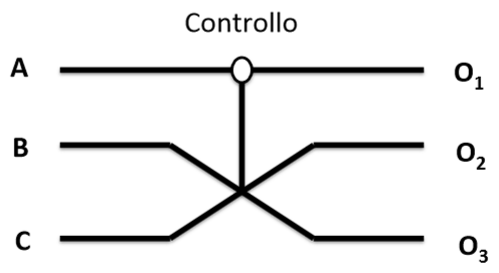
\includegraphics[width=0.4\textwidth]{Immagini/fredkin_circuit.png}
\end{center}
\section{Operazioni Bit-a-Bit}
A una stringa di $n$ bit possiamo associare un intero compreso fra 0 e $N-1$ con $N=2^n$. All'intero $x$ associamo la stringa di bit $x_0x_1x_2\dots x_{n}$ con $x_{i}=0,1 \text{ e } i=0,1,\dots,n$ tale che $x=\sum_{i=0}^{n}x_{i}2^{n-i}$.
\subsection{Prodotto interno bit-per-bit}
\begin{equation*}
    x\cdot z \equiv (x_{1}z_{1} + x_{2}z_{2} + \dots + x_{n}z_{n}) \mod 2
\end{equation*}
E' anche chiamato prodotto \texttt{AND} bitwise perchè si ottiene prendendo le operazioni \texttt{AND} fra i singoli bit.
\subsection{Somma bit-per-bit: bitwise \texttt{XOR}}
Indichiamo con $x\oplus z$ la somma bit-per bit, modulo 2. Il risultato questa volta è una stringa il cui $i$-esimo bit ha il valore $x_{i}+z_{i} \mod 2 = x_{i} \text{ \texttt{XOR} } z_{i}$.
\chapter{Apparato matematico}
\section{Prerequisiti matematici}
\subsection{Numeri complessi}
Ogni numero complesso $z\in \mathbb{C}$ può essere scritto come $z=a+ib$, con $a\in \mathbb{R}$ \textbf{parte reale} e $b\in \mathbb{R}$ \textbf{parte immaginaria}. Se $z=a+ib$ e $w=c+id$, abbiamo
\begin{equation*}
    z+w = (a+c) + i(b+d)
\end{equation*}
\begin{equation*}
    z\cdot w = (ac-bd) + i(ad+bc)
\end{equation*}
Per ogni $z\in \mathbb{C}$, $z\cdot z^{*}=a^{2}+b^{2}$ è reale e non negativo dove $z^{*}$ è il \textbf{complesso coniugato} di $z$ ($z^{*}=a-ib$). Inoltre, $\sqrt{a^{2}+b^{2}}=\lvert z\rvert$ è detto \textbf{modulo} di $z$.
\begin{equation*}
    \lvert z\rvert^{2} = z\cdot z^{*}
\end{equation*}
Possiamo rappresentare un numero complesso $z=a+ib$ come una coppia (a,b) sul piano complesso. L'asse delle ascisse è utilizzato per la parte reale e l'asse delle ordinate per la parte immaginaria. Si ha $a = \lvert z \rvert \cos \theta$ e $b = \lvert z \rvert \sin \theta$ dove $\theta$ è la \textbf{fase}. Se $z=0$ allora $\theta$ non è definita. Per $\lvert z \rvert = 1, z=\cos\theta + i\sin\theta$. Più in generale possiamo scrivere $z=\rho e^{i\theta}$ con $\rho=\lvert z \rvert$ e $e^{i\theta}=\cos\theta + i\sin\theta$.
\begin{equation*}
    i*(-i) = 1
\end{equation*}
\subsection{Spazi vettoriali in 2D}
\begin{itemize}
    \item \textbf{Direzione}: rappresentata dalla retta su cui giace il vettore
    \item \textbf{Verso}:  specifica in che direzione punta il vettore
\end{itemize}
Se abbiamo due vettori $u$ e $v$ possiamo definire la somma che sarà un vettore $w=u+v$ ottenuto mediante la \textbf{regola del parallelogramma}.\\
Dato un numero $\alpha\in \mathbb{R}$, per ogni vettore $v$, possiamo definire il vettore $\alpha v$ è la freccia ottenuta moltiplicando $v$ per $|\alpha|$ invertendone il verso se $\alpha < 0$. Questa operazione è detta \textbf{moltiplicazione per scalare}. Quindi se $\alpha = -1$, otteniamo il vettore $-v$ che ha stesso modulo, stessa direzione ma verso opposto a $v$.\\
L'insieme di tutti i vettori del piano è allora uno spazio vettoriale reale $V$ chiuso rispetto all'operazione di combinazione lineare:
\begin{equation*}
    u = \alpha v + \beta w
\end{equation*}
Per ogni vettore $v$ e $w \in V$ e per ogni $\alpha, \beta \in \mathbb{R}$.
\subsection{Prodotto scalare e componenti}
\begin{equation*}
    < \cdot, \cdot > : V \times V \rightarrow \mathbb{C}
\end{equation*}
Che soddisfa le seguenti proprietà:
\begin{enumerate}
    \item $\forall u\in V, <u,u>$ è un numero reale non negativo, con $<u,u>=0 \iff u=0$
    \item $\forall u,v \in V, <u,v>=<v,u>^{*}$
    \item $\forall u,v,w \in V,\forall \alpha,\beta \in \mathbb{C}, <w,\alpha u+\beta v>=\alpha<w,u>+\beta<w,v>$
\end{enumerate}
Due vettori per i quali il prodotto scalare è nullo sono \textit{ortogonali}, sono base ortonormali se sono ortogonali e a norma unitaria ($\lVert <\cdot,\cdot>\rVert_{2}=1$).\\
Inoltre riscrivendo $u=u_{0}v_{0}+u_{1}v_{1}$ si ha:
\begin{equation*}
    \begin{split}
        <u,u>&=<u_{0}v_{0}+u_{1}v_{1},u_{0}v_{0}+u_{1}v_{1}>\\
        &=<u_{0}v_{0},u_{0}v_{0}>+<u_{0}v_{0},u_{1}v_{1}>+<u_{1}v_{1},u_{0}v_{0}>+<u_{1}v_{1},u_{1}v_{1}>\\
        &=u_{0}^{2}<v_{0},v_{0}>+u_{0}u_{1}<v_{0},v_{1}>+u_{1}u_{0}<v_{1},v_{0}>+u_{1}^{2}<v_{1},v_{1}>\\
        &=u_{0}^{2}+u_{1}^{2}
    \end{split}
\end{equation*}
Dove $u_{0}=<u,v_{0}>$ e $u_{1}=<u,v_{1}>$
\subsection{Vettori ket e bra}
\begin{itemize}
    \item \textbf{Ket}: vettore $u \rightarrow |u\rangle$
    \item \textbf{Bra}: vettore $u \rightarrow \langle u|$
\end{itemize}
Usando questa notazione il prodotto scalare si forma con \textit{braket}:
\begin{equation*}
    <u,v>=\langle u|v\rangle
\end{equation*}
Usando la scomposizione di $v$ in componenti:
\begin{itemize}
    \item $|v\rangle = u_{0}|v_{0}\rangle + u_{1}|v_{1}\rangle$
    \item $\langle v| = u_{0}^{*}\langle v_{0}| + u_{1}^{*}\langle v_{1}|$
\end{itemize}
\subsubsection{Delta di Kronecker}
\begin{equation*}
    <v_{i},v_{j}> = \delta_{ij} = \begin{cases}
        1 & \text{se } i=j \\
        0 & \text{se } i\neq j
    \end{cases}
\end{equation*}
Usando queste notazioni possiamo scrivere il prodotto scalare come:
\begin{equation*}
    \begin{split}
        \langle v|v\rangle & = (u_{0}^{*}\langle v_{0}| + u_{1}^{*}\langle v_{1}|)\cdot (u_{0}|v_{0}\rangle + u_{1}|v_{1}\rangle) \\
        & = |u_{0}|^{2} \langle v_{0}|v_{0}\rangle + u_{0}^{*}u_{1}\langle v_{0}|v_{1}\rangle + u_{1}^{*}u_{0}\langle v_{1}|v_{0}\rangle + |u_{1}|^{2}\langle v_{1}|v_{1}\rangle \\
        & = |u_{0}|^{2}\cdot 1 + u_{0}^{*}u_{1} \cdot 0 + u_{1}^{*}u_{0} \cdot 0 + |u_{1}|^{2} \cdot 1 \\
        & = |u_{0}|^{2} + |u_{1}|^{2} \\
        & = | |v\rangle |^{2}
    \end{split}
\end{equation*}
\subsection{Prodotto tensore}
Consideriamo ora due spazi vettoriali $V$ e $W$ con basi, rispettivamente, $A=\left\{|\alpha_{1}\rangle_{V},\ldots,|\alpha_{n}\rangle_{V}\right\}$ e $B=\left\{|\beta_{1}\rangle_{W},\ldots,|\beta_{m}\rangle_{W}\right\}$. Da questa scrittura deduciamo che $V$ è uno spazio vettoriale di dimensione $n$ e $W$ di dimensione $m$.\\
Il prodotto tensore di $V$ e $W$ viene indicato con $V\otimes W$ ha dimensione $\dim(V\otimes W)=n\text{ }m$  con la base costituita da $n\text{ }m$ elementi della forma $|\alpha_{i}\rangle_{V}\otimes|\beta_{j}\rangle_{W}$.\\
\textbf{La notazione $|\alpha_{i}\rangle_{V}\otimes|\beta_{j}\rangle_{W}$ può essere scritta come $|\alpha_{i}\beta_{j}\rangle$}.\\
Proprietà:
\begin{enumerate}
    \item $\forall \ket{v},\ket{v'} \in V, \ket{w} \in W \quad (\ket{v}+\ket{v'})\otimes\ket{w} = \ket{v}\otimes\ket{w}+\ket{v'}\otimes\ket{w}$
    \item $\forall\ket{v}\in V, \ket{w},\ket{w'}\in W \quad \ket{v}\otimes (\ket{w}+\ket{w'})=\ket{v}\otimes\ket{w}+\ket{v}\otimes\ket{w'}$
    \item $\forall\ket{v}\in V,\ket{w}\in W,\alpha \in \mathbb{C} \quad (\alpha\ket{v})\otimes\ket{w}=\ket{v}\otimes(\alpha\ket{w})=\alpha(\ket{v}\otimes\ket{w})$
\end{enumerate}
Se $V$ e $W$ ammettono prodotto scalare, allora $V\otimes W$ ammette un prodotto scalare definito come:
\begin{equation*}
    \braket{u}{u'}=(\bra{v}\otimes\bra{w})\cdot(\ket{v'}\otimes\ket{w'})=\braket{v}{v'}\cdot\braket{w}{w'} \in \mathbb{C}
\end{equation*}
Alcune "proprietà":
\begin{enumerate}
    \item $(\bra{\alpha_{1}}\otimes\bra{\beta_{2}})\cdot(\ket{\alpha_{1}}\otimes\ket{\beta_{2}}) = \braket{\alpha_{1}}{\alpha_{1}}\cdot\braket{\beta_{2}}{\beta_{2}}=1$
    \item $\left\{\ket{\alpha_{i}}\otimes\ket{\beta_{j}}\right\}$ è una base ortonormale $V\otimes W$ \begin{itemize}
        \item Se $\braket{\alpha_{i}}{\alpha_{k}}\cdot\braket{\beta_{j}}{\beta_{l}}=1 \rightarrow \text{normalizzati}$
        \item Se $\braket{\alpha_{i}}{\alpha_{k}}\cdot\braket{\beta_{j}}{\beta_{l}}=0 \rightarrow \text{ortogonali}$
    \end{itemize}
\end{enumerate}
\subsubsection{Esempio}
$\ket{v} = a\ket{\alpha_{1}}_{V}+b\ket{a_{2}}_{V}\in V$\\
$\ket{w} = c\ket{\beta_{1}}_{W}+d\ket{\beta_{2}}_{W}\in W$ 
\begin{equation*}
    \begin{split}
        \ket{v}\otimes\ket{w} & = (a\ket{\alpha_{1}}_{V}+b\ket{\alpha_{2}}_{V})\otimes(c\ket{\beta_{1}}_{W}+d\ket{\beta_{2}}_{W}) \\
        & = ac(\ket{\alpha_{1}}_{V}\otimes\ket{\beta_{1}}_{W})+ad(\ket{\alpha_{1}}_{V}\otimes\ket{\beta_{2}}_{W})+bc(\ket{\alpha_{2}}_{V}\otimes\ket{\beta_{1}}_{W})+bd(\ket{\alpha_{2}}_{V}\otimes\ket{\beta_{2}}_{W}) \\
        \bra{v}\otimes\bra{w} & = (a\bra{\alpha_{1}}_{V}+b\bra{\alpha_{2}}_{V})\otimes(c\bra{\beta_{1}}_{W}+d\bra{\beta_{2}}_{W}) \\
        & = ac(\bra{\alpha_{1}}_{V}\otimes\bra{\beta_{1}}_{W})+ad(\bra{\alpha_{1}}_{V}\otimes\bra{\beta_{2}}_{W})+bc(\bra{\alpha_{2}}_{V}\otimes\bra{\beta_{1}}_{W})+bd(\bra{\alpha_{2}}_{V}\otimes\bra{\beta_{2}}_{W})
    \end{split}
\end{equation*}
\footnotesize
\begin{equation*}
    \begin{split}
        (\bra{v}\otimes\bra{w})\cdot(\ket{v}\otimes\ket{w}) & = [(a\bra{\alpha_{1}}_{V}+b\bra{\alpha_{2}}_{V})\otimes(c\bra{\beta_{1}}_{W}+d\bra{\beta_{2}}_{W})]\cdot[(a\ket{\alpha_{1}}_{V}+b\ket{\alpha_{2}}_{V})\otimes(c\ket{\beta_{1}}_{W}+d\ket{\beta_{2}}_{W})] \\
        & = \\
        & = (|a|^{2}+|b|^{2})\cdot(|c|^{2}+|d|^{2})
    \end{split}
\end{equation*}
\normalsize
\subsection{Operatori lineari}
Gli operatori lineari in generale sono tali che agendo su un vettore dello spazio lineare danno un altro vettore dello stesso spazio: $O:V\rightarrow V$. Usando la notazione braket possiamo scrivere \begin{equation*}
    O\ket{v}=\ket{w}
\end{equation*}
Scegliamo una base (ortonormale) dello spazio vettoriale $\left\{\ket{\alpha_{1}},\ldots,\ket{\alpha_{n}}\right\}$, l'elemento della matrice $O$ in posizione $(i,j)$ sarà $O_{ij}=\bra{\alpha_{i}}\cdot(O\ket{\alpha_{j}})$
\subsubsection{Esempio}
Voglio calcolare $O_{12}$:
\begin{equation*}
    \begin{split}
        O_{12} & =\bra{\alpha_{1}}\left(\sum_{ij}^{n}O_{ij}\ket{\alpha_{i}}\bra{\alpha_{j}}\right)\ket{\alpha_{2}}\\
        & = \sum_{ij}^{n} O_{ij}\braket{\alpha_{1}}{\alpha_{i}}\braket{\alpha_{j}}{\alpha_{2}} \\
        & = O_{12}
    \end{split}
\end{equation*}
Grazie al delta di Kronecker.
\subsection{Autovalori e Autovettori}
Diremo che se $O\ket{v}=\lambda\ket{v}$ per un vettore non nullo $\ket{v}$, diremo che $v$ è un \textbf{autovettore} di O e $\lambda$ è l'\textbf{autovalore} corrispondente.
\chapter{Introduzione ai fenomeni quantistici}
Un osservabile fisico può essere associato ad un operatore Hermittiano $\phi$ da cui possiamo ottenere i loro autovalori e autovettori. Il punto fondamentale di questa discussione è che la base, gli autovalori e il risultato dipende dall'osservabile che vogliamo misurare.
\section{Regole dal postulato della misura}
\begin{enumerate}
    \item Se vogliamo misurare un osservabile $\phi$, dobbiamo conoscere i suoi autovalori $\{\phi_{i}\}$ e autovettori $\{\ket{\phi_{i}}\}$; cioè gli stati tali che $\phi\ket{\phi_{i}}=\phi_{i}\ket{\phi_{i}}$. Gli autovettori saranno la base su cui decomporre lo stato del nostro sistema. Ovvero dobbiamo scrivere $\ket{a}=\sum_{i}a_{i}\ket{\phi_{i}}$ con $a_{i}=\braket{\phi_{i}}{a}$.
    \item La misura avrà come risultato l'autovalore $\phi_{i}$ con probabilità $|a_{i}|^{2}$.
    \item Dopo la misura, il sistema si troverà nello stato $\ket{\phi_{i}}$ associato all'autovalore misurato.
\end{enumerate}
Stati quantistici sono normalizzati:
\begin{equation*}
    \sum_{i=1}^{N}|a_{i}|^{2}=1
\end{equation*}
\section{Fase globale e relativa}
\subsection{Fase globale}
Consideriamo i vettori $\ket{u}$ e $e^{i\phi}\ket{u}$ che hanno lo stesso modulo ma differiscono per una fase globale $\phi$. Il calcolo delle probabilità dei risultati di una qualunque misura fornisce sempre gli stessi valori.\\
Sia $\ket{u}=\sum_{i}\alpha_{i}\ket{\phi_{i}}$ dove $\{\ket{\phi_{i}}\}$ formano una base ortonormale dello spazio vettoriale. Lo stato con una fase globale si scriverà $e^{i\phi}\ket{u}=\sum_{i}e^{i\phi}\alpha_{i}\ket{\phi_{i}}$
\subsubsection{Esempio di fase globale/relativa}
\begin{equation*}
    \tikzmark{ephi}e^{i\phi}\frac{(\ket{0}+\tikzmark{ephigamma}e^{i(\gamma - \phi)}\ket{1})}{\sqrt{2}}
\end{equation*}
\begin{tikzpicture}[overlay, remember picture]
    \node (ephi-desc) [below of= ephi] {Fase globale};
    \draw[<-] (ephi.south)++(.25em,-.5ex) -- (ephi-desc);
    \node (ephigamma-desc) [above of= ephigamma] {Fase relativa};
    \draw[<-] (ephigamma.north)++(.25em,2ex) -- (ephigamma-desc);
\end{tikzpicture}
\section{Stati a molti qubit}
\begin{itemize}
    \item \textbf{Base del qubit}: $\{\ket{0},\ket{1}\}$
    \item \textbf{Stato}: $\ket{\psi}=\alpha\ket{0}+\beta\ket{1}$
\end{itemize}
Consideriamo:
\begin{equation}
    \begin{split}
        &\text{A: } \ket{\psi} = \alpha\ket{0}+\beta\ket{1} \\
        &\text{B: } \ket{\phi} = \gamma\ket{0}+\delta\ket{1}
    \end{split}
\end{equation}
La base $B$ la otteniamo con:
\begin{equation*}
    \begin{split}
        \ket{\psi}\oplus\ket{\phi} &= \left(\alpha\ket{0}+\beta\ket{1}\right)\oplus\left(\gamma\ket{0}+\delta\ket{1}\right)\\
        &= \alpha\gamma\ket{00}+\alpha\delta\ket{01}+\beta\gamma\ket{10}+\beta\delta\ket{11}
    \end{split}
\end{equation*}
Per ricavare la base ci fermiamo al secondo passaggio, quindi avremo $B:\left\{\ket{00},\ket{01},\ket{10},\ket{11}\right\}$.
\subsection{Stati a due qubit separabili}
Usando $\ket{\psi}$ e $\ket{\phi}$ (3.1), a volte conviene scrivere lo stato come:
\begin{equation*}
    \ket{\psi}\oplus\ket{\phi} = \alpha\ket{0} \oplus \left(\gamma\ket{0}+\delta\ket{1}\right) + \beta\ket{1} \oplus \left(\gamma\ket{0}+\delta\ket{1}\right)
\end{equation*}
Perchè in questo modo si possono determinare le probabilità di collasso in modo più semplice:
\begin{equation*}
    \begin{cases}
        \text{Se collassa $\alpha$: } |\alpha|^{2},\phi_{0} \rightarrow \ket{0}\oplus\left(\gamma\ket{0}+\delta\ket{1}\right) = \begin{cases}
            \text{Se collassa $\gamma$: } |\gamma|^{2},\phi_{0}\rightarrow \ket{00}\\
            \text{Se collassa $\delta$: } |\delta|^{2},\phi_{1}\rightarrow \ket{01}
        \end{cases}\\
        \text{Se collassa $\beta$: } |\beta|^{2},\phi_{1} \rightarrow \ket{1}\oplus\left(\gamma\ket{0}+\delta\ket{1}\right) = \begin{cases}
            \text{Se collassa $\gamma$: } |\gamma|^{2},\phi_{0}\rightarrow \ket{10}\\
            \text{Se collassa $\delta$: } |\delta|^{2},\phi_{1}\rightarrow \ket{11}
        \end{cases}\\
    \end{cases}
\end{equation*}
\subsubsection{Esempio}
\begin{equation*}
    \begin{split}
        \ket{\varepsilon} &= \frac{1}{\sqrt{2}}\left(\ket{01}+\ket{10}\right) ?= \ket{\psi} \oplus \ket{\phi} \\
        &= \frac{1}{\sqrt{2}}\left(\ket{01}\right) + \frac{1}{\sqrt{2}}\left(\ket{10}\right) = \begin{cases}
            \text{Se collassa $\ket{01}$: } \frac{1}{2}, \phi_{0} \rightarrow \ket{01} \rightarrow 1,\phi_{0} \rightarrow \ket{01}\\
            \text{Se collassa $\ket{10}$: } \frac{1}{2}, \phi_{1} \rightarrow \ket{10} \rightarrow 1,\phi_{1} \rightarrow \ket{10}
        \end{cases}
    \end{split}
\end{equation*}
Possiamo dedurre che se A misura 0, B misura 1 e viceversa.
\subsection{Stati a due qubit entangled}
Gli elementi dello spazio vettoriale $A\oplus B$ non sono tutti ottenibili come prodotto tensoriale di due elementi di $A$ e $B$. \\
Un esempio di stati entangled sono gli stati di Bell:
\begin{equation*}
    \begin{split}
        &\ket{\phi^{+}} = \frac{1}{\sqrt{2}}\left(\ket{0}_{A}\oplus\ket{0}_{B}+\ket{1}_{A}\oplus\ket{1}_{B}\right) \\
        &\ket{\phi^{-}} = \frac{1}{\sqrt{2}}\left(\ket{0}_{A}\oplus\ket{0}_{B}-\ket{1}_{A}\oplus\ket{1}_{B}\right) \\
        &\ket{\psi^{+}} = \frac{1}{\sqrt{2}}\left(\ket{0}_{A}\oplus\ket{1}_{B}+\ket{1}_{A}\oplus\ket{0}_{B}\right) \\
        &\ket{\psi^{-}} = \frac{1}{\sqrt{2}}\left(\ket{0}_{A}\oplus\ket{1}_{B}-\ket{1}_{A}\oplus\ket{0}_{B}\right) \\
    \end{split}
\end{equation*}
Per descrivere lo stato di un sistema a due qubit possiamo alternativamente usare la base canonica $\left\{\ket{00},\ket{01},\ket{10},\ket{11}\right\}$ o la base di Bell $\left\{\ket{\phi^{+}},\ket{\phi^{-}},\ket{\psi^{+}},\ket{\psi^{-}}\right\}$.
\begin{equation*}
    O = \lambda_{0}\ket{\phi^{+}}\braket{\phi^{+}}[+\lambda_{1}]{\phi^{-}}\braket{\phi^{-}}[+\lambda_{2}]{\psi^{+}}\braket{\psi^{+}}[+\lambda_{3}]{\psi^{-}}\bra{\psi^{-}}
\end{equation*}
Quindi se il sistema si trova in uno stato di Bell, una misura dell'operatore $O$ darà con certezza l'autovalore corrispondente.
\section{Trasformazioni unitarie}
Sia $\ket{a} = \alpha\ket{x_{0}}+\beta\ket{x_{1}}$, una trasformazione  unitaria $U$ è
\begin{itemize}
    \item \textbf{Lineare}: $U\ket{a}=U(\alpha\ket{x_{0}}+\beta\ket{x_{1}}) = \alpha U\ket{x_{0}}+\beta U\ket{x_{1}}$
    \item \textbf{Invertibile  con l'inversa uguale alla trasposta coniugata}: $U^{-1}\ket{a}=U^{\dagger}\ket{a}$
\end{itemize}
Quest'ultima proprietà garantisce che le trasformazioni unitarie lasciano invariati i prodotti scalari, e quindi anche la norma dei vettori su cui agiscono e le probabilità associate alle misure. Infatti, prendiamo due stati $\ket{a}$ e $\ket{b}$ con prodotto scalare $\braket{b}{a}$. Se questi evolvono secondo un operatore unitario $U$ avremo $\ket{a'}=U\ket{a}$ e $\ket{b'}=U\ket{b}$ ($\bra{b'}=\bra{b}U^{\dagger}$), il prodotto scalare degli stati evoluti sarà $\braket{b'}{a'}=\braket{b}[U^{\dagger}U]{a}=\braket{b}{a}$ perchè $U^{\dagger}U=\text{Identità}$.
\subsection{Porte quantistiche}
\subsubsection{Trasformazioni di Pauli}
Nel nostro caso scegliamo la base canonica $\left\{\ket{0},\ket{1}\right\}$ e definiamo, oltre all'identità $Id$, le tre trasformazioni di Pauli $X,Y,Z$:
\begin{equation*}
    \begin{alignedat}{2}
        Id\ket{0} &\,:=\, \ket{0} \quad & Id\ket{1} &\,:=\, \ket{1} \\
        X\ket{0}  &\,:=\, \ket{1} \quad & X\ket{1}  &\,:=\, \ket{0} \\
        Y\ket{0}  &\,:=\,-i\ket{1} \quad & Y\ket{1} &\,:=\, i\ket{0} \\
        Z\ket{0}  &\,:=\,-\ket{0} \quad & Z\ket{1} &\,:=\, \ket{1}
    \end{alignedat}
\end{equation*}
Analizzando l'effetto degli operatori, si nota che nella base canonica, $X$ corrisponde al \texttt{NOT} tra bit classici. L'operatore $Z$ genera un cambio della fase relativa e, infine, l'operatore $Y$ può essere visto come una combinazione dei due precedenti dato che $Y=-iXZ$.\\
\textbf{Esempio}
\begin{equation*}
    \begin{split}
        Z\left(\alpha\ket{0}+\beta\ket{1}\right) &= \alpha Z\ket{0}+\beta Z\ket{1} \\
        &= -\alpha\ket{0}+\beta\ket{1}
    \end{split}
\end{equation*}
\subsubsection{Trasformazioni di Hadarmard}
\begin{equation*}
    \begin{split}
        H\ket{0} &= \ket{+} = \frac{(\ket{0}+\ket{1})}{\sqrt{2}} \\
        H\ket{1} &= \ket{-} = \frac{(\ket{0}-\ket{1})}{\sqrt{2}}
    \end{split}
\end{equation*}
In forma matriciale (nella base canonica $\left\{\ket{0},\ket{1}\right\}$) l'operatore di Hadarmard si scrive come:
\begin{equation*}
    H = \frac{1}{\sqrt{2}}
    \begin{pmatrix}
        1 & 1 \\
        -1 & 1
    \end{pmatrix}
\end{equation*}
\subsubsection{Controlled-NOT}
Consideriamo ora, il controlled-NOT, \texttt{CNOT}, una trasformazione che agisce su 2 qubit, $A$ e $B$. Nella base canonica l'azione del \texttt{CNOT} é:
\begin{equation*}
    \begin{split}
        CNOT \ket{0}_{A}\oplus \ket{0}_{B} &= \ket{0}_{A}\oplus \ket{0}_{B} \\
        CNOT \ket{0}_{A}\oplus \ket{1}_{B} &= \ket{0}_{A}\oplus \ket{1}_{B} \\
        CNOT \ket{1}_{A}\oplus \ket{0}_{B} &= \ket{1}_{A}\oplus \ket{1}_{B} \\
        CNOT \ket{1}_{A}\oplus \ket{1}_{B} &= \ket{1}_{A}\oplus \ket{0}_{B} 
    \end{split}
\end{equation*}
In linea generale possiamo scrivere il \texttt{CNOT} come:
\begin{equation*}
    C_{i}NOT_{j}
\end{equation*}
Dove $i$ è il qubit di controllo e $j$ il qubit target. Se il qubit di controllo è acceso allora applica un \texttt{NOT} al qubit target.\\
L'importanza dell'operatore \texttt{CNOT} risiede nel fatto che può generare entanglement fra due qubit.\\
\textbf{Esempio}
\begin{equation*}
    \ket{00} \xrightarrow{H_{1}} \frac{\ket{0}+\ket{1}}{\sqrt{2}} \oplus \ket{0} = \frac{1}{\sqrt{2}}\left(\ket{00}+\ket{10}\right) \xrightarrow{C_{1}NOT_{2}} \frac{1}{\sqrt{2}}\left(\ket{00}+\ket{11}\right) = \text{Stato di Bell}
\end{equation*}
\customfbox{Se eseguo l'operatore \texttt{CNOT} due volte ottengo lo stato iniziale: \begin{equation*}
    CNOT^{2} = Id
\end{equation*}}
\section{Sfera di Bloch}
Come detto un generico stato quantistico a due livelli o qubit è scritto come $\ket{v}=\alpha\ket{0}+\beta\ket{1}$ con il vincolo ulteriore di normalizzazione dello stato: $\lvert \alpha \rvert^{2} + \lvert \beta \rvert^{2} = 1$. Quindi in generale possiamo scrivere $\lvert \alpha \rvert^{2}=\cos^{2}\left(\theta\right) \rightarrow \lvert \alpha \rvert=\cos\left(\frac{\theta}{2}\right)$ e $\lvert \beta \rvert^{2}=\sin^{2}\left(\theta\right) \rightarrow \lvert \beta \rvert=\sin\left(\frac{\theta}{2}\right)$
Possiamo rappresentare gli stati dei qubit in modo geometrico. Consideriamo lo stato generico
\begin{equation*}
    \ket{\psi} = \cos\left(\frac{\theta}{2}\right)\ket{0}+\sin\left(\frac{\theta}{2}\right)e^{i\phi}\ket{1}
\end{equation*}
e il relativo stato bra
\begin{equation*}
    \bra{\psi} = \cos\left(\frac{\theta}{2}\right)\bra{0}+\sin\left(\frac{\theta}{2}\right)e^{-i\phi}\bra{1}    
\end{equation*}
Calcoliamo i valori medi degli operatori di Pauli $X,Y,Z$ con lo stato $\ket{\psi}$
\begin{equation*}
    \begin{split}
        x &= \braket{\psi}[X]{\psi} = \cos \phi \sin \theta \\
        y &= \braket{\psi}[Y]{\psi} = \sin \phi \sin \theta \\
        z &= \braket{\psi}[Z]{\psi} = \cos \theta \text{ (oppure $-\cos \theta$)}
    \end{split}
\end{equation*}
Queste non sono altro che le coordinate in uno spazio tridimensionale di un punto che si muove su una sfera. Se consideriamo il vettore che congiunge l'origine degli assi con il punto di coordinate $\{x,y,z\}$, l'angolo $\theta$ è quello formato dal vettore e dall'asse $z$ mentre l'angolo $\phi$ è quello formato dal vettore sul piano $y-z$
\begin{center}
    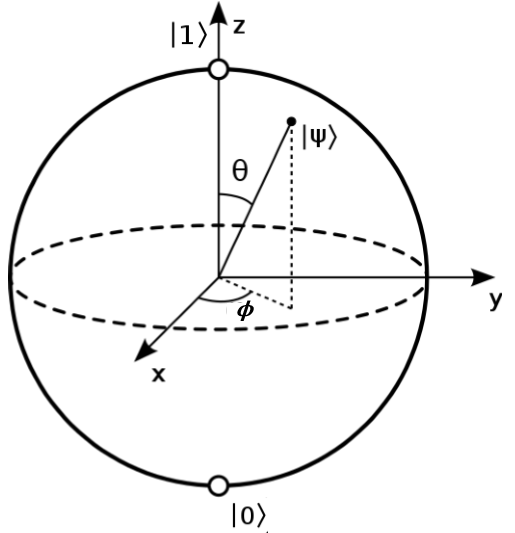
\includegraphics[width=0.5\textwidth]{Immagini/sferadibloch.png}
\end{center}
Concludiamo che ogni operatore unitario può essere visto come una rotazione sulla sfera di Bloch che unisce lo stato iniziale con lo stato finale.\\
L'operatore $U$ possiamo scriverlo più generalmente come:
\begin{equation*}
    U = \cos\left(\frac{\alpha}{2}\right)Id - i\sin\left(\frac{\alpha}{2}\right)Y
\end{equation*}
\textbf{Esempio}
\begin{equation*}
    \begin{split}
        \ket{\psi} &= \ket{1} \\
        \ket{\psi_{f}} &= U\ket{\psi} \\
        &= \cos\left(\frac{\alpha}{2}\right)Id\ket{1}-i\sin\left(\frac{\alpha}{2}\right)Y\ket{1} \\
        &= \cos\left(\frac{\alpha}{2}\right)\ket{1}-i\sin\left(\frac{\alpha}{2}\right)i\ket{0} \\
        &= \cos\left(\frac{\alpha}{2}\right)\ket{1}+\sin\left(\frac{\alpha}{2}\right)\ket{0} \\
    \end{split}
\end{equation*}
\chapter{Informazione Quantistica}
\section{Parallelismo quantistico}
Supponiamo di partire dai due qubit inizializzati nello stato $\ket{00}\equiv\ket{0}\otimes\ket{0}$ e di applicare due porte di Hadarmard ai singoli qubit. Le due porte applicate contemporaneamente si denotano come $H\otimes H\equiv H^{\otimes 2}$ dove la notazione $\otimes$ indica che la prima porta è applicata al primo qubit e la seconda al secondo qubit
\begin{equation*}
    \begin{split}
        \ket{0}\otimes\ket{0}\xrightarrow{H^{\otimes 2}} \frac{\ket{0}+\ket{1}}{\sqrt{2}}\otimes\frac{\ket{0}+\ket{1}}{\sqrt{2}} &= \frac{\ket{00}}{2}+\frac{\ket{01}}{2}+\frac{\ket{10}}{2}+\frac{\ket{11}}{2} \\
        &= \frac{1}{2}\left(\ket{00}+\ket{01}+\ket{10}+\ket{11}\right)
    \end{split}
\end{equation*}
Se applichiamo un operatore unitario $U$
\begin{equation*}
    \begin{split}
        \frac{1}{2}\left(\ket{00}+\ket{01}+\ket{10}+\ket{11}\right)\xrightarrow{U}\frac{1}{2}\left(U\ket{00}+U\ket{01}+U\ket{10}+U\ket{11}\right)
    \end{split}
\end{equation*}
Ovvero agirà contemporaneamente su tutti gli stati logici. Questo ragionamento si estende in maniera semplice al caso di $n$ qubit. In questo caso lo stato iniziale sarà $\ket{00\ldots 0}$ e applicheremo $n$ porte di Hadarmard $H^{\otimes n}$
\begin{equation*}
    \begin{split}
        \ket{00\ldots 0} \xrightarrow{H^{\otimes n}} \frac{\ket{0}+\ket{1}}{\sqrt{2}}\otimes\dots\otimes\frac{\ket{0}+\ket{1}}{\sqrt{2}} &= \frac{1}{2^{\frac{n}{2}}}\left(\ket{00\ldots 0}+\ket{10\ldots 0}+\ldots+\ket{11\ldots 1}\right) \\
        &= \frac{1}{\sqrt{N}}\sum_{x=0}^{N-1}\ket{x}
    \end{split}
\end{equation*}
Dove $N=2^{n}$ e anche in questo caso, applicando successivamente un operatore unitario $U$ avremo
\begin{equation*}
    \frac{1}{\sqrt{N}}\sum_{x=0}^{N-1}U\ket{x}
\end{equation*}
Possiamo manipolare parallelamente tutte le $N$ stringhe logiche.
\section{Teorema no-cloning}
Supponiamo di avere un singolo qubit di informazione e che si trovi nello stato $\ket{\psi}=a\ket{0}+b\ket{1}$ (con $|a|^{2}+|b|^{2}=1$). Per copiarlo, prendiamo un secondo qubit inizializzato nello stato $\ket{0}$. Avremo $\ket{\psi0}=a\ket{00}+b\ket{10}$ e applichiamo la porta \texttt{CNOT}
\begin{equation*}
    \ket{\psi0}=a\ket{00}+b\ket{10}\xrightarrow{C_{1}NOT_{2}} a\ket{00}+b\ket{11}
\end{equation*}
Se consideriamo lo stato più generale $\ket{\psi0}=a\ket{00}+b\ket{10}$ per copiarlo dovremmo avere un operatore il cui risultato sia
\begin{equation*}
    \ket{\psi\psi} = a^{2}\ket{00}+ab\ket{01}+ab\ket{10}+b^{2}\ket{11}
\end{equation*}
\customfbox{Se lo stato da copiare è sconosciuto, non è possibile copiarlo.}
L'operazione di copiatura sarà descritta da un'evoluzione unitaria $U_{COPY}$ tale che
\begin{equation*}
    \ket{\psi s}\xrightarrow{U_{COPY}}\ket{\psi s}=\ket{\psi\psi}
\end{equation*}
Supponiamo di voler copiare anche uno stato $\ket{\varphi}$ 
\begin{equation*}
    \ket{\varphi s}\xrightarrow{U_{COPY}}\ket{\varphi s}=\ket{\varphi\varphi}
\end{equation*}
Se prendendo il prodotto scalare degli stati finali abbiamo
\begin{equation*}
    \braket{\varphi s}[U^{\dagger}_{COPY}U_{COPY}]{\psi s} = \braket{\varphi s}{\psi s} = \braket{\varphi}{\psi}\braket{s}{s} = \braket{\varphi}{\psi}
\end{equation*}
\textbf{Esempio}\\
$s = 0$
\begin{equation*}
    \begin{split}
      \bra{\varphi}\bra{0}U^{\dagger}_{COPY}\left(U_{COPY}\ket{\psi}\ket{0}\right) &= \bra{\varphi}\bra{0}I\ket{\psi}\ket{0} \\
      &= \left(\bra{\varphi}\bra{0}\right)\left(\ket{\psi}\ket{0}\right) \\
      &= \braket{\varphi}{\psi}\braket{0}{0} \\
      &= \braket{\varphi}{\psi}
    \end{split}
\end{equation*}
Dalle equazioni di sopra, questo deve essere uguale a $\braket{\psi\psi}{\varphi\varphi} = \braket{\varphi}{\psi}\braket{\varphi}{\psi}$
\begin{equation*}
    \braket{\varphi}{\psi} = \left(\braket{\varphi}{\psi}\right)^{2}
\end{equation*}
Quindi può esistere un operatore unitario di copia $U_{COPY}$ solo se gli stati $\ket{psi}$ e $\ket{\varphi}$ sono ortogonali ($\braket{\varphi}{\psi} = 0$) oppure identici ($\braket{\varphi}{\psi} = 1$).\\
Concludiamo che se gli stati da copiare sono noti e ortogonali è possibile costruire un operatore unitario $U_{COPY}$ che li copi. In genere, però non è possibile copiare stati quantistici qualsiasi; ovvero non esiste nessun operatore $U_{COPY}$ capace di copiare tutti gli stati quantistici. 
\section{Superdense coding}
Supponiamo che Alice voglia mandare due bit di informazione classica. Alice e Bob devono condividere uno stato entangled (di Bell)
\begin{equation*}
    \ket{\beta_{00}} = \frac{1}{\sqrt{2}}\left(\ket{0}_{A}\otimes\ket{0}_{B}+\ket{1}_{A}\otimes\ket{1}_{B}\right)
\end{equation*}
Dove gli stati $\ket{\ldots}_{A}$ e $\ket{\ldots}_{B}$ sono rispettivamente di Alice e Bob.
\begin{center}
    \begin{tabular}{| c | c | c |}
        \hline
        \textbf{Bit di Alice} & \textbf{Porta logica applicata} & \textbf{Stato di Bob} \\
        \hline
        00 & $I$ & $\frac{\left(\ket{00}_{B}+\ket{11}_{B}\right)}{\sqrt{2}} \xrightarrow{C_{1}NOT_{2}} \frac{\left(\ket{00}_{B}+\ket{10}_{B}\right)}{\sqrt{2}} \xrightarrow{H} \ket{00}_{B}$ \\
        \hline
        01 & $X$ & $\frac{\left(\ket{10}_{B}+\ket{01}_{B}\right)}{\sqrt{2}} \xrightarrow{C_{1}NOT_{2}} \frac{\left(\ket{11}_{B}+\ket{01}_{B}\right)}{\sqrt{2}} \xrightarrow{H} \ket{01}_{B}$ \\
        \hline
        10 & $Z$ & $\frac{\left(\ket{00}_{B}-\ket{11}_{B}\right)}{\sqrt{2}} \xrightarrow{C_{1}NOT_{2}} \frac{\left(\ket{00}_{B}-\ket{10}_{B}\right)}{\sqrt{2}} \xrightarrow{H} \ket{10}_{B}$ \\
        \hline
        11 & $iY$ & $\frac{\left(\ket{01}_{B}-\ket{10}_{B}\right)}{\sqrt{2}} \xrightarrow{C_{1}NOT_{2}} \frac{\left(\ket{01}_{B}-\ket{11}_{B}\right)}{\sqrt{2}} \xrightarrow{H} \ket{11}_{B}$ \\
        \hline
    \end{tabular}
\end{center}
\section{Teletrasporto quantistico}
Supponiamo che Alice (A) e Bob (B) condividano uno stato entangled $\ket{\beta_{00}} = \frac{\ket{00}+\ket{11}}{\sqrt{2}}$. Questa notazione sta per la più precisa
\begin{equation*}
    \ket{\beta_{00}} = \frac{1}{\sqrt{2}}\left(\ket{0}_{A}\otimes\ket{0}_{B}+\ket{1}_{A}\otimes\ket{1}_{B}\right) = \frac{1}{\sqrt{2}}\left(\ket{00}+\ket{11}\right)
\end{equation*}
Supponiamo che Alice abbia aun qubit di informazione $\ket{\psi} = \alpha\ket{0}+\beta\ket{1}$ (con $\lvert \alpha \rvert^{2}+\lvert \beta \rvert^{2}=1$) che vuole mandare a Bob. Per far questo, lo accoppia allo stato entangled $\ket{\beta_{00}}$
\begin{equation*}
    \ket{\psi_{0}} = \ket{\psi}\ket{\beta_{00}} = \frac{1}{\sqrt{2}}\left[\alpha\ket{0}(\ket{00}+\ket{11})+\beta\ket{1}(\ket{00}+\ket{11})\right]
\end{equation*}
Dove si intende, ad esempio, $\ket{0}\ket{00}=\ket{0}_{A}\ket{0}_{A}\ket{0}_{B}$.\\
Poi viene applicata una porta \texttt{CNOT} usando il primo qubit A come bit di controllo e il secondo qubit B come bit target (se vediamo i qubit come $\ket{000}$ sarebbe $C_{1}NOT_{3}$)
\begin{equation*}
    \ket{\psi_{0}} \xrightarrow{C_{1}NOT_{2}} \ket{\psi_{1}} = \frac{1}{\sqrt{2}}\left[\alpha\ket{0}(\ket{00}+\ket{11})+\beta\ket{1}(\ket{01}+\ket{10})\right]
\end{equation*}
Successivamente Alice applica una porta di Hadarmard al primo qubit
\begin{equation*}
    \begin{split}
        \ket{\psi_{1}} \xrightarrow{H_{1}} \ket{\psi_{2}}& = \frac{1}{2}\left[\alpha(\ket{0}+\ket{1})(\ket{00}+\ket{11})+\beta(\ket{0}-\ket{1})(\ket{01}+\ket{10})\right] \\ &
        = \frac{1}{2}\left[\ket{00}(\alpha\ket{0}+\beta\ket{1})+\ket{01}(\alpha\ket{1}+\beta\ket{0})+\ket{10}(\alpha\ket{0}-\beta\ket{1})+\ket{11}(\alpha\ket{1}-\beta\ket{0})\right]
    \end{split}
\end{equation*}
l'ultimo passo è quindi quello di rendere tale informazione accessibile a Bob. Per fare questo, Alice misura i suoi due qubit e dato che i qubit di Alice e Bob sono entangled, la  misura di Alice induce un collasso dello stato di Bob. I possibili risultati della misura di Alice e i corrispondenti stati di Bob sono
\begin{center}
    \begin{tabular}{| c | c | c | c |}
        \hline
        \textbf{Misura} & \textbf{Stato di Bob} & \textbf{Probabilità di misurare 0} & \textbf{Probabilità di misurare 1}\\
        \hline
        00 & $\alpha\ket{0}+\beta\ket{1}$ & $\mathcal{P}_{00}(0) = \lvert \alpha \rvert^{2}$ & $\mathcal{P}_{00}(1) = \lvert \beta \rvert^{2}$\\
        \hline
        01 & $\alpha\ket{1}+\beta\ket{0}$ & $\mathcal{P}_{01}(0) = \lvert \beta \rvert^{2}$ & $\mathcal{P}_{01}(1) = \lvert \alpha \rvert^{2}$\\
        \hline
        10 & $\alpha\ket{0}-\beta\ket{1}$ & $\mathcal{P}_{10}(0) = \lvert \alpha \rvert^{2}$ & $\mathcal{P}_{10}(1) = \lvert \beta \rvert^{2}$\\
        \hline
        11 & $\alpha\ket{1}-\beta\ket{0}$ & $\mathcal{P}_{11}(0) = \lvert \beta \rvert^{2}$ & $\mathcal{P}_{11}(1) = \lvert \alpha \rvert^{2}$\\
        \hline
    \end{tabular}
\end{center}
Ognuno di queste misure capita con probabilità di $\frac{1}{4}$. Affinchè Bob possegga sempre lo stato $\ket{\psi} = \alpha\ket{0}+\beta\ket{1}$, Alice chiama attraverso un canale classico Bob e gli dice quale è stato il risultato della sua misura. A questo punto Bob applica un'operatore correttivo
\begin{center}
    \begin{tabular}{| c | c |}
        \hline
        \textbf{Misura} & \textbf{Operatore correttivo} \\
        \hline
        00 & $I$ \\
        \hline
        01 & $X$ \\
        \hline
        10 & $Z$ \\
        \hline
        11 & $Y$ \\
        \hline
    \end{tabular}
\end{center}
La probabilità totale di misurare 0 per Bob è
\begin{equation*}
    \begin{split}
        \mathcal{P}_{Bob}(0) &= \frac{1}{4}\left(\mathcal{P}_{00}(0)+\mathcal{P}_{01}(0)+\mathcal{P}_{10}(0)+\mathcal{P}_{11}(0)\right) \\
        &= \frac{1}{4}\left(\lvert \alpha \rvert^{2}+ \lvert \beta \rvert^{2} +\lvert \alpha \rvert^{2}+ \lvert \beta \rvert^{2}\right) \\
        &= \frac{1}{4}(1+1) = \frac{1}{2}
    \end{split}
\end{equation*}
Stessa cosa per $\mathcal{P}_{Bob}(1)=\frac{1}{2}$.\\
La conclusione è che sebbene Alice abbia modificato lo stato (o gli stati) di Bob, quest'ultimo non è in grado di estrarre nessuna informazione.
\section{Algoritmi quantistici}
\subsection{Algoritmo di Deutch}
Data una funzione $f$ ad un bit, l'algoritmo di Deutch permette di capire se sia costante o no; nel caso in cui $f$ non sia costante viene spesso chiamata \textbf{bilanciata}. Si consideri una funzione ad un bit $f(x):\{0,1\}\rightarrow\{0,1\}$, la funzione $f$ sarà costante se $f(0)=f(1)$ e sarà bilanciata se $f(0)\neq f(1)$.\\
Lo stato iniziale dell'algoritmo di Deutch è costituito da due qubit: $\ket{\psi_{0}}=\ket{01}$. Ad entrambi viene applicata una porta di Hadarmard per  ottenere
\begin{equation*}
    \ket{\psi_{0}}\rightarrow\ket{\psi_{1}} = \frac{1}{2}\left(\ket{0}+\ket{1}\right)\left(\ket{0}-\ket{1}\right)
\end{equation*}
\subsubsection{L'operatore $U_{f}$}
L'effetto di questo operatore è quello di calcolare $f(x)$, l'addizione modulo 2 di $y\oplus f(x)$ e lo possa immagazzinare nel secondo qubit ($\ket{x,y}\rightarrow\ket{x,y\oplus f(x)}$). L'addizione modulo 2 è equivalente ad una porta \texttt{XOR}.\\
Per capire come agisce l'operatore $U_{f}$, nell'algoritmo di Deutch, lo applichiamo ad uno stato generico $\ket{x}\ket{-}$:
\begin{equation*}
    \begin{split}
        \ket{x}\ket{-} = \ket{x}\frac{\ket{0}-\ket{1}}{\sqrt{2}} &\xrightarrow{U_{f}}_{x=0} \ket{0}\frac{\ket{0}-\ket{1}}{\sqrt{2}} = \frac{1}{\sqrt{2}}\left(\ket{00}-\ket{01}\right)\\
        &\xrightarrow{U_{f}} \frac{1}{\sqrt{2}}\left(\ket{0,0\oplus f(0)}-\ket{0,1\oplus f(0)}\right) = \begin{cases}
            \frac{1}{\sqrt{2}}\left(\ket{00}-\ket{01}\right) = \ket{0}\ket{-} & \text{se $f(0)=0$} \\
            \frac{1}{\sqrt{2}}\left(\ket{01}-\ket{00}\right) = -\ket{0}\ket{-} & \text{se $f(0)=1$}
        \end{cases}
    \end{split}
\end{equation*}
In sostanza, l'applicazione dell'operatore $U_{f}$ lascia invariato sia il primo qubit che il secondo ma lo stato acquista una fase $(-1)^{f(x)}$ che dipende dal  valore della funzione $f$ calcolata per $x$:
\begin{equation*}
    \ket{x}\frac{\ket{0}-\ket{1}}{\sqrt{2}}\rightarrow(-1)^{f(x)}\ket{x}\frac{\ket{0}-\ket{1}}{\sqrt{2}}
\end{equation*} 
Possiamo dire che lo stato $\ket{x}\frac{\ket{0}-\ket{1}}{\sqrt{2}}$ è un autovettore dell'operatore $U_{f}$ con autovalore $(-1)^{f(x)}$.\\
Tornando allo stato iniziale $\ket{\psi_{1}}$, applichiamo l'operatore $U_{f}$ e una porta di Hadarmard sul primo qubit per ottenere
\begin{equation*}
    \begin{split}
        \ket{\psi_{2}} = U_{f}\ket{\psi_{1}} &= \frac{1}{\sqrt{2}}\left((-1)^{f(0)}\ket{0}+(-1)^{f(1)}\ket{1}\right) \\ 
        &\xrightarrow{H_{1}} \frac{1}{2}\left[\ket{0}\left((-1)^{f(0)}+(-1)^{f(1)}\right)+\ket{1}\left((-1)^{f(0)}-(-1)^{f(1)}\right)\right]
    \end{split}
\end{equation*}
Se la funzione è costante avremo che $(-1)^{f(0)}+(-1)^{f(1)}=2$ e $(-1)^{f(0)}-(-1)^{f(1)}=0$ quindi $\ket{\psi_{2}}=\ket{0}$. Al contrario se la funzione è bilanciata avremo che $(-1)^{f(0)}+(-1)^{f(1)}=0$ e $(-1)^{f(0)}-(-1)^{f(1)}=\pm2$ quindi $\ket{\psi_{2}}=\pm\ket{1}$ e visto che il segno $\pm$ può essere visto come fase globale, possiamo dire che lo stato finale è $\ket{1}$.
\customfbox{L'algoritmo di Deutch permette di migliorare le performance dell'algoritmo classico perchè usa il parallelismo quantistico.}
\subsection{Algoritmo di Deutch-Josza}
L'algoritmo di Deutch-Josza segue i passaggi dell'algoritmo di Deutch. Lo stato iniziale è
\begin{equation*}
    \ket{\psi_{0}} = \ket{0}^{\otimes n}\ket{1}
\end{equation*}
Vengono applicate $n+1$ porte di Hadarmard ai primi $n+1$ qubit. In questo modo otteniamo la sovrapposizione di tutte le stringhe di bit con gli interi da 0 a $N-1 = 2^{n}-1$. Lo stato diviene
\begin{equation*}
    \ket{\psi_{1}} = \frac{1}{\sqrt{N}}\sum_{x=0}^{N-1}\ket{x}\ket{-}
\end{equation*} 
A questo punto a questo stato viene applicato l'operatore $U_{f}$ (da Bob) che si comporta così $U_{f}:\ket{x,y}\rightarrow\ket{x,y\oplus f(x)}$  e quindi
\begin{equation*}
    \ket{\psi_{2}} = \frac{1}{\sqrt{N}}\sum_{x=0}^{N-1}(-1)^{f(x)}\ket{x}\ket{-}
\end{equation*}
Successivamente Alice applica $n$ porte di Hadarmard ai primi $n$ qubit. Per capire come queste agiscono, è utile considerare il singolo qubit $\ket{k}$ con $k=\{0,1\}$. Conosciamo il risultato dal calcolo diretto ma è utile scriverlo in maniera compatta come
\begin{equation*}
    H\ket{k} = \frac{1}{\sqrt{2}}\sum_{z=0}^{1}(-1)^{kz}\ket{z}
\end{equation*}
Estendendo questo ragionamento a tutti gli $n$ qubit, otteniamo
\begin{equation*}
    H^{\otimes n}\ket{x_{1},x_{2},\ldots,x_{n}} = \sum_{x_{1},x_{2},\ldots,x_{n}}^{1}\frac{(-1)^{x_{1}z_{1}+x_{2}z_{2}+\ldots+x_{n}z_{n}}}{\sqrt{N}}\ket{z_{1},z_{2},\ldots,z_{n}}
\end{equation*}
Che può essere riscritta in maniera compatta come:
\begin{equation*}
    H^{\otimes n}\ket{x} = \sum_{z=0}^{N-1}\frac{(-1)^{x\cdot z}}{\sqrt{N}}\ket{z}
\end{equation*}
Ora riscriviamo lo stato $\ket{\psi}$
\begin{equation*}
    \ket{\psi_{2}} = \sum_{x=0}^{N-1}\sum_{z=0}^{N-1} \frac{(-1)^{x\cdot z + f(x)}}{N}\ket{z}\ket{-}
\end{equation*}
Se $z=0$ sappiamo che $x\cdot z = 0$ e se $f$ costante ($f(x)\rightarrow \bar{f}$ ) per tutti i valori di $x$ allora il termine $(-1)^{f(x)}$ non dipende più da $x$
\begin{equation*}
    \sum_{x=0}^{N-1} \frac{(-1)^{\bar{f}}}{N} = (-1)^{\bar{f}}\sum_{x=0}^{N-1} \frac{1}{N} = (-1)^{\bar{f}}
\end{equation*}
Quindi se la funzione è costante
\begin{equation*}
    \ket{\psi_{2}} = \ket{0}\ket{-}
\end{equation*}
e una misura dei primi $n$ qubit restituirà sempre 0.\\
Se la funzione è bilanciata non possiamo portare fuori il fattore $(-1)^{f(x)}$ però sappiamo che per $\frac{N}{2}$ stringhe varrà $+1$ ($f(x)=0$) e per le altre $\frac{N}{2}$ varrà $-1$ ($f(x)=1$). Quindi il coefficiente dello stato $\ket{0}$ sarà
\begin{equation*}
    \sum_{x=0}^{N-1} \frac{(-1)^{f(x)}}{N} = \left(\sum_{f(x)=0}\frac{1}{N}\right)-\left(\sum_{f(x)=1}\frac{1}{N}\right) = \frac{1}{N}\left(\frac{N}{2}-\frac{N}{2}\right) = 0
\end{equation*}
\subsection{Algoritmo di Bernstein-Vazirani}
Supponiamo di avere uno spazio logico a $n$ bit e di avere una funzione che per ogni input $x$ calcola $f_{a}(x)=x\cdot a = x_{1}a_{1}+x_{2}a_{2}+\ldots+x_{n}a_{n}$ dove la stringa a $n$ bit $a$ è ignota. L'obiettivo è quello di determinare la stringa $a$.\\
L'azione dell'oracolo non sarà quello di aggiungere una fase $(-1)^{f(x)}$ ma una fase $(-1)^{x\cdot a}$ ($f_{a}(x)=x\cdot a$).
\begin{equation*}
    \begin{split}
        \ket{\psi_{2}} &= \sum_{x=0}^{N-1}\sum_{z=0}^{N-1} \frac{(-1)^{x\cdot z+x\cdot a}}{N}\ket{z}\ket{-} \\
        &= \sum_{x=0}^{N-1}\sum_{z=0}^{N-1} \frac{(-1)^{(z\oplus a)\cdot x}}{N}\ket{z}\ket{-} \\
        &= \sum_{z=0}^{N-1}\left(\sum_{x=0}^{N-1} \frac{(-1)^{(z\oplus a)\cdot x}}{N}\right)\ket{z}\ket{-} \\
        &= \sum_{z=0}^{N-1}X_{z}\ket{z}\ket{-}
    \end{split}
\end{equation*}
Se $z=a$ vuol dire che le due stringhe hanno tutti gli $n$ bit uguali ($z_{i}=a_{i}$). Per l'$i$-esimo bit dovremmo alcolare $z_{i}\text{\texttt{ XOR }}a_{i}$.\\
Il passo successivo è calcolare $(z+a)\cdot x$ che darà 0 visto che per i singoli bit avremo $(z_{i}+a_{i})\cdot x_{i}=0$ di conseguenza abbiamo che 
\begin{equation*}
    X_{z=a}=\sum_{x=0}^{N-1} \frac{1}{N} = 1
\end{equation*}
e quindi tutti gli altri coefficienti devono essere annullati $X_{z\neq a}=0$
\subsection{Algoritmo di Simon}
\customfbox{
    \begin{equation*}
        f: \{0,1\}^{n} \rightarrow \{0,1\}^{n}
    \end{equation*}
}
La funzione $f$ ha la caratteristica che per ogni $x$ esiste un solo $y$ tale che $f(x)=f(y)$. Tale $y$ non è casuale ma sappiamo che è calcolato secondo la regola $y=x\oplus a$ dove $a$ è una stringa di $n$ bit. L'obiettivo è quello di determinare la stringa $a$, ovvero, la periodicità della funzione $f$.\\
L'unica possibilità che abbiamo è di dare all'oracolo una serie di stringhe fino a che non troviamo una coppia $x$ e $y$ tale che $f(x)=f(y)$. Una volta trovate tali stringhe, il periodo può essere calcolato come $a=x\oplus y$.\\
In media sono necessari $2^{\frac{n}{2}}$ tentativi e chiamate dell'oracolo. Supponiamo come nell'algoritmo di Deutch-Josza di partire da $n$ bit logici più $n$ qubit addizionali $\ket{\psi_{0}}=\ket{0}^{\otimes n}\ket{0}^{\otimes n}$ e di applicare $N$ porte di Hadarmard ai primi $n$ qubit:
\begin{equation*}
    \ket{\psi_{1}} = \frac{1}{\sqrt{N}}\sum_{x=0}^{N-1}\ket{x}\ket{0}^{\otimes n}
\end{equation*}
Dato che $\ket{0\oplus f(x)} = \ket{f(x)}$
\begin{equation*}
    \ket{\psi_{1}} \xrightarrow{O} \ket{\psi_{2}} = \frac{1}{\sqrt{N}}\sum_{x=0}^{N-1} \ket{x}\ket{f(x)}
\end{equation*}
Dato che per ogni $x$ esiste un $x\oplus a$ tale che $f(x)=f(x\oplus a)$, possiamo scrivere
\begin{equation*}
    \ket{\psi_{2}} = \frac{1}{\sqrt{\frac{N}{2}}} \sum_{x=0}^{N-1}\frac{\ket{x}+\ket{x\oplus a}}{\sqrt{2}}\ket{f(x)}
\end{equation*}
$f(x)$ collassa a $f(x_{0})$ con probabilità $\frac{1}{2^{n-1}}=\frac{2}{N}$ e il valore di questa stringa non è importante quindi possiamo scrivere lo stato come
\begin{equation*}
    \ket{\psi_{3}}=\frac{\ket{x_{0}}+\ket{x_{0}\oplus a_{0}}}{\sqrt{2}}
\end{equation*}
Applichiamo $n$ porte di Hadarmard
\begin{equation*}
    \begin{split}
        \frac{\ket{x_{0}}+\ket{x_{0}\oplus a}}{\sqrt{2}} &\xrightarrow{H^{\otimes n}} \frac{1}{\sqrt{2}}\left(\frac{1}{\sqrt{N}}\sum_{z=0}^{N-1}(-1)^{x_{0}\cdot z}\ket{z} + \frac{1}{\sqrt{N}}\sum_{z=0}^{N-1}(-1)^{(x_{0}\oplus a)\cdot z}\ket{z}\right)\\
        &= \frac{1}{\sqrt{2}}\left(\frac{1}{\sqrt{N}}\sum_{z=0}^{N-1}(-1)^{x_{0}\cdot z}\ket{z} + \frac{1}{\sqrt{N}}\sum_{z=0}^{N-1}(-1)^{x_{0}\cdot z + a\cdot z}\ket{z}\right) \\
        &= \frac{1}{\sqrt{2N}}\left(\sum_{z=0}^{N-1}(-1)^{x_{0}\cdot z}\left(1+(-1)^{a\cdot z}\right)\ket{z}\right)
    \end{split}
\end{equation*}
Il prodotto interno bit-per-bit $a\cdot z = \{0,1\}$ per le stringhe $z$ per cui $a\cdot z=1$, il coefficiente dello stato $\ket{z}$ è 0. Al contrario se $a\cdot z=0$ il coefficiente è 1. La possiamo riscrivere come:
\begin{equation*}
    \ket{\psi_{4}} = \frac{1}{\sqrt{2N}} \sum_{a\cdot z=0} (-1)^{x_{0}\cdot z}\left[1+(-1)^{a\cdot z}\right]\ket{z}
\end{equation*}
Dobbiamo iterare la procedura per ottenere diversi valori $z_{2},z_{3},\ldots,z_{n}$ tali che $a\cdot z_{i}=0$ per $i=1,\ldots,n$. Con questi $z_{i}$ possiamo risolvere il sistema di equazioni
\begin{equation*}
    \begin{cases}
        a\cdot z_{1} = 0 \\
        a\cdot z_{2} = 0 \\
        \vdots \\
        a\cdot z_{n} = 0
    \end{cases}
\end{equation*}
Se le equazioni sono linearmente indipendenti esiste una sola stringa $a$ che le soddisfa tutte e può essere facilmente determinata.
\chapter{Crittografia quantistica}
La crittografia quantistica segue uno schema a chiave privata e, in  particolare, si focalizza sullo scambio delle chiavi private (si parla infatti di Quantum Key Distribution o QKD).
\section{Protocollo BB84}
Il protocollo BB84 è un protocollo sicuro per la distribuzione di chiavi crittografiiche. Un eventuale hacker (Eve) non può copiare un generico qubit contenente l'informazione a causa del teorema no-cloning e non può misurare un qubit senza pertubarlo a causa del collasso della funzione d'onda.\\
Per il protocollo  BB84 possiamo identificare due basi indicate con $B_{1}$ e $B_{2}$:
\begin{itemize}
    \item $B_{1}:\{\ket{0},\ket{1}\}$
    \item $B_{2}: \{\ket{+},\ket{-}\}$
\end{itemize}
\subsection{Implementazione}
\begin{enumerate}
    \item La prima sequenza $n$ rappresenta una stringa logica associata al messaggio mentre la seconda rappresenta la base in cui codificare il messaggio. 
    \begin{center}
        \begin{tabular}{c c c c c c}
            \textbf{Logica} & 0 & 1 & 1 & 0 & 1  \\
            \textbf{Basi} & 0 & 0 & 1 & 0 & 0  \\
            \textbf{Messaggio} & $\ket{0}$ & $\ket{1}$ & $\ket{-}$ & $\ket{0}$ & $\ket{1}$  \\
        \end{tabular}
    \end{center}
    \item L'output è certo dato che le stringhe delle basi di Alice e Bob coincidono.
    \item Alice e Bob pubblicano apertamente le stringhe delle basi e poi guardano quali sono i bit con le basi in comune e creano la chiave a partire da quei bit.
    \begin{center}
        \textbf{Alice}
        \begin{tabular}{c c c c c}
            0 & 1 & 1 & 0 & 1  \\
            0 & 0 & 1 & 0 & 0  \\
            $\ket{0}$ & $\ket{1}$ & $\ket{-}$ & $\ket{0}$ & $\ket{1}$  \\
        \end{tabular}\\
        \vspace{0.5em}
        \textbf{Bob}
        \begin{tabular}{c c c c c}
            1 & 0 & 1 & 1 & 0  \\
            0 & 0 & 1 & 0 & 0  \\
            $\ket{1}$ & $\ket{0}$ & $\ket{-}$ & $\ket{1}$ & $\ket{0}$  \\
        \end{tabular}
    \end{center}
\end{enumerate}
\textbf{Intervento di Eve}\\
Visto che Eve non può copiare i qubit per il teorema no-cloning, l'unica cosa che può  fare è inserirsi nella comunicazione fra Alice e  Bob e sostituirsi a Bob nella misura per poi mandare a Bob dei qubit.
\section{Protocollo B92}
Invece di scegliere due basi, Alice ne sceglie solo una $B=\{\ket{0},\ket{+}\}$. Gli stati della base $B$ sono non-ortogonali dato che $\braket{0}{+}=\frac{1}{\sqrt{2}}$.
\begin{enumerate}
    \item Come nel BB84, Alice estrae una sola stringa di $n$ numeri random. Se Alice ha estratto 0 costruirà il qubit $\ket{0}$; se ha estratto 1 costruirà il qubit $\ket{+}$. In seguito, li invia a Bob tramite un canale quantistico.
    \item Ricevuti i qubit Bob estrae una stringa di $n$ numeri random e fa una misura. La misura viene fatta nella base $B_{1}=\{\ket{0},\ket{1}\}$ se ha estratto 0 e nella base $B_{2}=\{\ket{+},\ket{-}\}$ se ha estratto 1. \begin{enumerate}
        \item Se Bob sceglie la base $B_{1}$ (estrae 0) e misura lo stato $\ket{1}$, sa immediatamente che Alice ha mandato il qubit $\ket{+}$ e quindi ha lo stato logico 1.
        \item Se Bob sceglie la base $B_{1}$ e misura lo stato $\ket{0}$, questo potrebbe essere associato allo stato di Alice $\ket{0}$ o $\ket{+}$. Quindi Bob non riesce a risalire al valore del qubit di Alice.
        \item Se Bob sceglie la base $B_{2}$ e misura lo stato $\ket{-}$, sa immediatamente che Alice ha mandato il qubit $\ket{0}$ e quindi ha lo stato logico 0.
        \item Se Bob sceglie la base $B_{2}$ e misura lo stato $\ket{+}$, questo potrebbe essere associato allo stato di Alice $\ket{0}$ o $\ket{+}$. Quindi Bob non riesce a risalire al valore del qubit di Alice.
    \end{enumerate}
    \item Bob pubblica la posizione dei bit per i quali non è certo del valore del bit di Alice. Questi bit vengono scartati e i rimanenti bit costituiranno la chiave segreta dato che il loro valore non è stato pubblicato.
    \item Per capire se Eve ha intercettato i qubit, Alice e Bob pubblicano metà dei bit che sanno essere perfettamente correlati. Se c'è un disaccordo, sanno che Eve ha intercettato la comunicazione e ignorano la stringa scambiata.
\end{enumerate}
\section{Protocollo EPR con stati entangled}
Supponiamo che Alice  e Bob condividano $n$ qubit entangled come
\begin{equation*}
    \ket{\phi^{+}} = \frac{\ket{00}+\ket{11}}{\sqrt{2}}
\end{equation*}
Alice genera un bit random classico $b$ e, a seconda del suo valore, misura il suo qubit nella base $B_{1}$ o nella base $B_{2}$ (le stesse usata per il protocollo BB84). Supponiamo che il valore di questa misura sia $a$. Allo stesso modo, Bob genera un bit random classico $b'$.\\
Supponiamo che il bit random di Alice sia $b=0$ e che Alice misuri nella base $B_{1}$. Se misura 0 (il 50\% delle volte), il sistema collasserà nello stato $\ket{00}$. Se Bob estrae il numero $b'=0$ e misura nella base $B_{1}$, il suo risultato sarà 0 il 100\% delle volte. Allo stesso modo se Alice misura 1 il sistema  collassa nello stato $\ket{11}$ e se $b'=0$, Bob misurerà sempre 1. Ne consegue che $b=b'=0$ i qubit di Alice e Bob sono perfettamente correlati.\\
Supponiamo ora che Alice estragga il numero $b=1$ e decida di misurare nella base $B_{2}$. Abbiamo che lo stato entangled può essere scritto come
\begin{equation*}
    \begin{split}
        \ket{\phi^{+}} &= \frac{1}{\sqrt{2}}\left(\frac{\ket{+}+\ket{-}}{\sqrt{2}}\otimes\ket{0}+\frac{\ket{+}-\ket{-}}{\sqrt{2}}\otimes\ket{1}\right) \\
        &= \frac{1}{\sqrt{2}}\left(\ket{+}\otimes\frac{\ket{0}+\ket{1}}{\sqrt{2}}+\ket{-}\otimes\frac{\ket{0}-\ket{1}}{\sqrt{2}}\right) \\
        &= \frac{\ket{++}+\ket{--}}{\sqrt{2}}   
    \end{split}
\end{equation*}
Seguendo il ragionamento precedente è chiaro che se Bob estrae $b'=1$, le misure di Alice e Bob sono perfettamente correlate. Ovvero, se il qubit di Alice collassa in $\ket{\pm}$ anche quello di Bob si trovera nello stato $\ket{\pm}$.\\
Supponiamo che Alice abbia $b=0$ e $b'=1$ e che la misura di Alice faccia collassare i qubit nello stato $\ket{00}$
\begin{equation*}
    \ket{00}=\ket{0}\otimes\frac{\ket{+}+\ket{-}}{\sqrt{2}}
\end{equation*}
E' chiaro che una misura di Bob nella base $B_{2}$ darà metà delle volte lo stato $\ket{+}$ e il risultato $a'=0$ e la rimanente metà lo stato $\ket{-}$ e il risultato $a'=1$.
\section{Quantum Money}
Lo scopo è quello di sfruttare la meccanica quantistica per costruire una moneta che non possa essere contraffatta.\\
La moneta quantistica è costituita da $n$ qubit $M_{n}$ a cui associa un numero intero di serie $0\leq m_{n} \leq 2^{n}-1$. Come nel BB84 la prima stringa rappresenta l'informazione logica mentre la seconda è la stringa delle basi quantistiche $B_{m}$: si usa la base $B_{1}$ quando nella seconda stringa compare  lo stato 0 e la base $B_{2}$ quando compare lo stato 1. Viene invece conservato il numero di serie $m_{n}$ associato alla stringa delle basi $B_{m}$ e alla stringa della moneta $M_{n}$.\\
\textbf{Esempio:}
\begin{center}
    \begin{tabular}{c c c c}
        0 & 1 & 0 & 1 \\
        0 & 0 & 1 & 1 \\
        $\ket{0}$ & $\ket{1}$ & $\ket{+}$ & $\ket{-}$ \\
    \end{tabular}
\end{center}
\textbf{La terza riga è la nostra moneta quantistica}.\\
Per certificare l'autenticità della moneta, Alice invia la moneta alla banca che l'ha emessa. La banca controlla il numero di serie $m_{n}$, risale alla stringa delle basi quantistiche $B_{m}$ e, usando quest'ultima, fa una misura nelle corrispondenti basi. Se la moneta è quella corretta, tutte le misure saranno deterministiche e la banca riotterà la stringa $M_{n}$.\\
\textit{Pensandola come tabella:}
\begin{center}
    \begin{tabular}{| c | c | c |}
        \hline
        \textbf{id} & \textbf{stringa logica} & \textbf{stringa basi} \\
        \hline
        $m_{n}$ & ****** & ****** \\
        \hline
    \end{tabular}
\end{center}
Dove l'id è pubblico mentre le stringhe sono private e solo la banca può vederle.
\chapter{Algoritmi quantistici}
\section{Algoritmo di Grover per la ricerca in database}
\subsection{Oracolo o Black box}
Supponiamo di avere un database di $N=2^{n}$ elementi con $n$ bit. Gli interi associati saranno nell'intervallo compreso fra 0 e $N-1$.\\
Tutta l'informazione sul problema che vogliamo risolvere è codificata in una funzione $f$ che ha come input un intero $x$ (o una stringa di $n$ bit) e come output un singolo bit. In altre parole, $f:\{0,1\}^{\otimes n}\rightarrow\{0,1\}$. Per definizione, $f(x)=1$ se $x$ è soluzione del nostro problema e $f(x)=0$ altrimenti.\\
Supponiamo che ci sia dato un numero intero $m$ e che ci sia detto che è il prodotto di due numeri primi $p$ e $q$: $m=p\cdot q$. Dobbiamo trovare quali sono $p$ e $q$. In questo caso la funzione $f$ implementata dall'oracolo non fa  altro che prendere un intero $x$ come input, dividere $m$ per $x$ e controllare se la divisione è esatta. Quindi l'oracolo non conosce la soluzione ma è in grado di verificare velocemente se un numero è soluzione o no del problema.\\
Allo stato generico $\ket{x}$ associamo un qubit aggiuntivo detto spesso qubit oracolo o \textbf{ancilla} $\ket{q}$, sarà quindi $\ket{x}\ket{q}$
\begin{equation*}
    \ket{x}\ket{q} \xrightarrow{O} \ket{x}\ket{q\oplus f(x)}
\end{equation*}
Se $q=0$ e se $x$ è soluzione, $f(x)=1$ e $\ket{0\oplus 1} = \ket{1}$. Al contrario se $x$ non è soluzione, $f(x)=0$ e $\ket{0\oplus 0} = \ket{0}$.
\begin{equation*}
    \ket{x}\ket{0}\xrightarrow{O}\begin{cases}
        \ket{x}\ket{1} & \text{se $x$ è soluzione} \\
        \ket{x}\ket{0} & \text{se $x$ non è soluzione}
    \end{cases}
\end{equation*} 
Se $q=1$ e se $x$ è soluzione, $f(x)=1$ e $\ket{1\oplus 1} = \ket{0}$. Al contrario se $x$ non è soluzione, $f(x)=0$ e $\ket{1\oplus 0} = \ket{1}$.
\begin{equation*}
    \ket{x}\ket{0}\xrightarrow{O}\begin{cases}
        \ket{x}\ket{0} & \text{se $x$ è soluzione} \\
        \ket{x}\ket{1} & \text{se $x$ non è soluzione}
    \end{cases}
\end{equation*} 
Questa osservazione ci permette di studiare in altri casi dove il qubit ancilla nello stato $\ket{q}=\ket{-}$. Lo stato totale si può scrivere come
\begin{equation*}
    \ket{x}\otimes\ket{-} = \frac{1}{\sqrt{2}}\left(\ket{x}\otimes\ket{0}-\ket{x}\otimes\ket{1}\right) \xrightarrow{O}\begin{cases}
        \frac{1}{\sqrt{2}}\left(\ket{x}\otimes\ket{1}-\ket{x}\otimes\ket{0}\right) & \text{se $x$ è soluzione} \\
        \frac{1}{\sqrt{2}}\left(\ket{x}\otimes\ket{0}-\ket{x}\otimes\ket{1}\right) & \text{se $x$ non è soluzione} \\
    \end{cases}
\end{equation*}
I due stati ottenuti differiscono solo per un segno meno che possiamo fattorizzare come una fase
\begin{equation*}
    \ket{x}\otimes\ket{-}\xrightarrow{O}(-1)^{f(x)}\ket{x}\otimes\ket{-}
\end{equation*}
Se usando $q=0$, lo stato $\ket{x}\ket{q}$ viene modificato, usando $\ket{q}=\ket{-}$ acquista solo una fase $(-1)^{f(x)}$ mentre la struttura non viene cambiata. In quest'ultimo caso possiamo addirittura dimenticarci del qubit ancilla (visto che non viene modificato ed è uguale per tutti gli stati $\ket{x}$) e scrivere l'effetto solo sui qubit logici:
\begin{equation*}
    \ket{x}\xrightarrow{O}(-1)^{f(x)}\ket{x}
\end{equation*}
\subsection{Algoritmo di Grover}
L'algoritmo di Grover inizia con la costruzione dello stato quantistico sovrapposizione di tutti i possibili stati logici, può essere costruito partendo dallo stato di soli zeri $\ket{00\ldots  0}$ con l'applicazione di $n$ porte di Hadarmard:
\begin{equation*}
    \ket{\psi} = \frac{1}{\sqrt{N}}\sum_{x=0}^{N-1}\ket{x}
\end{equation*}
\subsubsection{Implementazione dell'operatore di Grover $G$}
\begin{enumerate}
    \item Applicare allo stato l'oracolo che cambia la fase allo stato soluzione: \begin{equation*}
        \ket{x}\xrightarrow{O}(-1)^{f(x)}\ket{x}
    \end{equation*}
    \item Applicare $n$ porte di Hadarmard
    \item Applicare un cambio di fase a tutti gli stati tranne allo stato $\ket{00\ldots 0}$: \begin{equation*}
        \ket{x}\xrightarrow{O}(-1)^{\delta_{x_{0}}}\ket{x}
    \end{equation*} dove $\delta_{x_{0}}$ è il delta di Kronecker ovvero $\ket{0}\rightarrow\ket{0}$ e per $x\neq 0$, $\ket{x}\rightarrow -\ket{x}$
    \item Applicare $n$ porte di Hadarmard
\end{enumerate}
L'algoritmo per la ricerca in un database si riduce alla sua applicazione per un numero $\sqrt{N}=2^{\frac{n}{2}}$ (tldr: applica $G$ per $\sqrt{N}$ volte).
\subsection{Stati "soluzione" e "non-soluzione"}
Lo spazio logico può essere diviso in due sottospazi. Quello generato da $\ket{x}$ con $x$ soluzione del nostro problema ($S$) e quelli che non sono soluzione del nostro problema ($\bar{S}$). Supponiamo che ci siano $M$ stati soluzione e, di conseguenza, $N-M$ non-soluzione
\begin{equation*}
    \begin{split}
        \ket{\alpha} &= \frac{1}{\sqrt{N-M}}\sum_{x\in\bar{S}}^{\ket{x}} \\
        \ket{\beta} &= \frac{1}{\sqrt{M}}\sum_{x\in S}^{\ket{x}}
    \end{split}
\end{equation*}
Con questa notazione lo stato iniziale $\ket{\psi}$ si scrive come
\begin{equation*}
    \begin{split}
        \ket{\psi} &= \frac{1}{\sqrt{N}}\left(\sum_{x\in S}\ket{x}+\sum_{x\in\bar{S}}\ket{x}\right) \\
        &= \frac{1}{\sqrt{N}}\left(\sqrt{M}\ket{\beta}+\sqrt{N-M}\ket{\alpha}\right) \\
        &= \sqrt{\frac{N-M}{N}}\ket{\alpha}+\sqrt{\frac{M}{N}}\ket{\beta}
    \end{split}
\end{equation*}
\subsection{Operatore di Grover}
Come detto l'oracolo cambia segno solo agli stati soluzione, quindi cambierà segno allo stato $\ket{\beta}$ lasciando $\ket{\alpha}$ invariato. Se lo facciamo agire su uno stato generico a $a\ket{\alpha}+b\ket{\beta}$ otteniamo
\begin{equation*}
    O\left(a\ket{\alpha}+b\ket{\beta}\right) = a\ket{\alpha}-b\ket{\beta}
\end{equation*}
Nella notazione braket:
\begin{equation*}
    O = \ket{\alpha}\bra{\alpha}-\ket{\beta}\bra{\beta}
\end{equation*}
E in termini di matrici:
\begin{equation*}
    O = \begin{bmatrix}
        1 & 0 \\
        0 & -1
    \end{bmatrix}
\end{equation*}
Per indicare l'operatore che cambia la fase a tutti tranne lo 0
\begin{equation*}
    U  = 2\ket{\bar{0}}\bra{\bar{0}}-I
\end{equation*}
Possiamo verificare che se $\ket{x}\neq\ket{\bar{0}}$
\begin{equation*}
    U\ket{x} = (2\ket{\bar{0}}\bra{\bar{0}}-I)\ket{x} = -\ket{x}
\end{equation*}
e che 
\begin{equation*}
    U\ket{\bar{0}} = (2\ket{\bar{0}}\bra{\bar{0}}-I)\ket{\bar{0}} = \ket{\bar{0}}
\end{equation*}
A questo punto possiamo scrivere la parte rimanente dell'operatore di Grover  come
\begin{equation*}
    H^{\otimes n}UH^{\otimes n} = 2\ket{\psi}\bra{\psi}-I
\end{equation*}
L'ultimo passaggio deriva dal fatto che $H^{\otimes n}\ket{\bar{0}}=\frac{1}{\sqrt{N}}\sum_{x=0}^{N-1}\ket{x}=0\ket{\psi}$ e che $H^{\otimes n}IH^{\otimes n}=I$.\\
Ne consegue che l'operatore di Grover può essere scritto come
\begin{equation*}
    G=\left(2\ket{\psi}\bra{\psi}-I\right)O
\end{equation*}
\subsection{Interpretazione geometrica}
Lo stato $\ket{\psi}$ è normalizzato e può essere riscritto in termini di funzioni seno e coseno come
\begin{equation*}
    \begin{split}
        \ket{\psi} &= \cos\left(\frac{\theta}{2}\right)\ket{\alpha}+\sin\left(\frac{\theta}{2}\right)\ket{\beta} \\
        \cos\left(\frac{\theta}{2}\right) &= \sqrt{\frac{N-M}{N}} \\
        \sin\left(\frac{\theta}{2}\right) &= \sqrt{\frac{M}{N}}
    \end{split}
\end{equation*}
Abbiamo che $\braket{\psi}{\alpha}=\cos\frac{\theta}{2}$ e $\braket{\psi}{\beta}=\sin\frac{\theta}{2}$.
\begin{equation*}
    \begin{split}
        (2\ket{\psi}\bra{\psi}-I)\ket{\alpha} &= 2\ket{\psi}\braket{\psi}{\alpha}-\ket{\alpha} \\
        &= 2\cos\frac{\theta}{2}\ket{\psi}-\ket{\alpha} \\
        &= 2\cos\frac{\theta}{2}\left(\cos\frac{\theta}{2}\ket{\alpha}+\sin\frac{\theta}{2}\ket{\beta}\right)-\ket{\alpha} \\
        &= \cos\theta\ket{\alpha}+\sin\theta\ket{\beta}
    \end{split}
\end{equation*}
In maniera del tutto analoga abbiamo
\begin{equation*}
    \begin{split}
        (2\ket{\psi}\bra{\psi}-I)\ket{\beta} &= 2\ket{\psi}\braket{\psi}{\beta}-\ket{\alpha} \\
        &= 2\cos\frac{\theta}{2}\ket{\psi}-\ket{\beta} \\
        &= 2\cos\frac{\theta}{2}\left(\cos\frac{\theta}{2}\ket{\alpha}+\sin\frac{\theta}{2}\ket{\beta}\right)-\ket{\beta} \\
        &= \sin\theta\ket{\alpha}-\cos\theta\ket{\beta}
    \end{split}
\end{equation*}
Questo ci permette di scrivere l'operatore $U$ in forma matriciale come
\begin{equation*}
    U=\begin{pmatrix}
        \braket{\alpha}[U]{\alpha} & \braket{\alpha}[U]{\beta} \\
        \braket{\beta}[U]{\alpha} & \braket{\beta}[U]{\beta}
    \end{pmatrix}
    =\begin{pmatrix}
        \cos\theta & \sin\theta \\
        \sin\theta & -\cos\theta
    \end{pmatrix}
\end{equation*}
Ne consegue che l'operatore di Grover nello spazio $\{\ket{\alpha},\ket{\beta}\}$ e in forma matriciale si scrive come
\begin{equation*}
    G = UO =
    \begin{pmatrix}
        \cos\theta & \sin\theta \\
        \sin\theta & -\cos\theta
    \end{pmatrix}
    \begin{pmatrix}
        1 & 0 \\
        0 & -1
    \end{pmatrix} =
    \begin{pmatrix}
        \cos\theta & -\sin\theta \\
        \sin\theta & \cos\theta
    \end{pmatrix}
\end{equation*}
Confermando l'osservazione che $G$ ruota lo stato di $\theta$.
\subsection{Effetto dell'operatore di Grover}
L'operatore di Grover nella rappresentazione è immediatamente associabile ad una rotazione nel piano definito dagli stati $\ket{\alpha}$ e $\ket{\beta}$.\\
Per capire meglio questo punto, supponiamo di applicarlo allo stato $\ket{\phi}=\cos\delta\ket{\alpha}+\sin\delta\ket{\beta}$
\begin{equation*}
    G\ket{\phi} = \begin{pmatrix}
        \cos\theta & -\sin\theta \\
        \sin\theta & \cos\theta
    \end{pmatrix}\cdot \begin{pmatrix}
        \cos\delta \\
        \sin\delta
    \end{pmatrix} = \begin{pmatrix}
        \cos(\delta+\theta) \\
        \sin(\delta+\theta)
    \end{pmatrix}
\end{equation*}
Se applichiamo $k$ volte l'operatore di Grover, genereremo nello spazio $\{\ket{\alpha}.\ket{\beta}\}$ una rotazione di un angolo $k\theta$
\begin{equation*}
    G^{k} = \begin{pmatrix}
        \cos k\theta & -\sin k\theta \\
        \sin k\theta & \cos k\theta
    \end{pmatrix}
\end{equation*}
Se lo stato iniziale è $\ket{\psi}= \cos\left(\frac{\theta}{2}\right)\ket{\alpha}+\sin\left(\frac{\theta}{2}\right)\ket{\beta}$ e applichiamo $G$ per $k$ volte otteniamo
\footnotesize
\begin{equation*}
    G^{k}\ket{\psi} = \begin{pmatrix}
        \cos k\theta & -\sin k\theta \\
        \sin k\theta & \cos k\theta
    \end{pmatrix}\begin{pmatrix}
        \cos\left(\frac{\theta}{2}\right) \\
        \sin\left(\frac{\theta}{2}\right)
    \end{pmatrix} =
    \begin{pmatrix}
        \cos\left(\frac{\theta}{2}+k\theta\right) \\
        \sin\left(\frac{\theta}{2}+k\theta\right)
    \end{pmatrix} =
    \cos\left(\frac{\theta}{2}+k\theta\right)\ket{\alpha}+\sin\left(\frac{\theta}{2}+k\theta\right)\ket{\beta}
\end{equation*}
\normalsize
\subsection{Performace dell'algoritmo di Grover}
Per avere la certezza di misurare uno degli stati in $\ket{\beta}$ dobbiamo avere
\begin{equation*}
    \sin\left(\frac{\theta}{2}+k\theta\right) \approx 1
\end{equation*}
Che equivale a dire
\begin{equation*}
    \frac{\theta}{2}+k\theta \approx \frac{\pi}{2}
\end{equation*}
Quindi
\begin{equation*}
    \begin{split}
        \frac{\theta}{2}+k\theta &\approx \frac{\pi}{2} \\
        k\theta &\approx \frac{\pi}{2}-\frac{\theta}{2} \\
        k\theta &\approx \frac{1}{2}(\pi-\theta) \\
        k &\approx \frac{1}{2}\left(\frac{\pi}{\theta}-1\right)
    \end{split}
\end{equation*}
Che valore assume $\theta$? Sappiamo che $\sin\frac{\theta}{2}=\sqrt{\frac{M}{N}}$ nei casi in cui ci sono poche soluzioni. Quindi $\frac{\theta}{2}$ sarà molto piccolo e per lo sviluppo della serie di Taylor avremo che:
\begin{equation*}
    \begin{split}
        \sin\frac{\theta}{2}\approx\frac{\theta}{2}&=\sqrt{\frac{M}{N}}\\
        \theta &= 2\sqrt{\frac{M}{N}}
    \end{split}
\end{equation*}
Usando questa approssimazione possiamo scrivere
\begin{equation*}
    \begin{split}
        k &\approx \frac{1}{2}\left(\frac{\pi}{\theta}-1\right) \\
        k &\approx \frac{1}{2}\left(\frac{\pi}{2\sqrt{\frac{M}{N}}}-1\right) \\
        k &\approx \frac{1}{2}\left(\frac{\pi}{2}\sqrt{\frac{N}{M}}-1\right) \\
        k &\approx \frac{\pi}{4}\sqrt{\frac{N}{M}} \\
    \end{split}
\end{equation*}
\chapter{Introduzione ai codici di correzione degli errori per computer quantistici}
\section{Correzione degli erorri nei computer classici}
Se, ad esempio, immagazziniamo in un hardisk o mandiamo attraverso una rete una stringa di bit, è possibile che l'inevitabile rumore generi dei \textbf{bit flip} ovvero trasformi alcuni bit che inizialmente avevano valore 0 in bit con valore 1 e viceversa.\\
Uno dei metodi più semplici e allo stesso tempo più efficaci per ovviare a questi errori è quello di  misurare tutti i bit e usare il protocollo di \textit{voto di maggioranza}: se la maggioranza dei bit ha valore 0 assumiamo che il bit logico sia 0 e correggiamao l'errore trovato; analogamente, se la maggioranza dei bit ha valore 1 assumiamo che il bit logico sia 1.
\customfbox{
    Ad esempio il bit logico 0 può essere codificato come 000 e il bit logico 1 può essere codificato come 111
}
Da questo è chiaro che il numero di bit usai deve essere dispari.
\section{Caso quantistico: i problemi}
\begin{itemize}
    \item Come nel caso classico, il bit flip corrisponde alla transizione $\ket{0}\rightarrow\ket{1}$ e viceversa.
    \item \textbf{Errori piccoli} in cui il sistema non ha una transizione completa ma transisce verso una sovrapposizione di stati; per esempio: $\ket{0}\rightarrow\gamma\ket{0}+\delta\ket{1}$
    \item La fase relativa fra gli stati può essere modificata per effetto del rumore; per esempio, $\alpha\ket{0}+\beta\ket{1}\rightarrow\alpha\ket{0}+e^{i\phi}\beta\ket{1}$
\end{itemize}
\section{Codici di correzione degli errori quantistici}
Il più semplice codice di correzione degli errori quantistici sfrutta, come l'analogo classico, il voto di maggioranza.\\
Definiamo i qubit logici come stati composti da un numero dispari di qubit fisici:
\begin{equation*}
    \begin{split}
        \ket{0_{L}} &\equiv \ket{000} \\
        \ket{1_{L}} &\equiv \ket{111}
    \end{split}
\end{equation*}
Lo stato quantistico generico sarà dunque scritto come $\alpha\ket{0_{L}}+\beta\ket{1_{L}}$ e si può ottenere a partire dallo stato a singolo qubit con delle semplici porte \texttt{CNOT}:
\begin{equation*}
    (\alpha\ket{0}+\beta\ket{1})\otimes\ket{0}\xrightarrow{C_{1}NOT_{2}}(\alpha\ket{00}+\beta\ket{11})\otimes\ket{0}\xrightarrow{C_{1}NOT_{3}}\alpha\ket{000}+\beta\ket{111}
\end{equation*}
Si noti che una misura diretta dello stato distruggerebbe la sovrapposizione e quindi parte dell'informazione. E' necessario quindi trovare degli osservabili che permettano di estrarre l'informazione desiderata senza perturbare  lo stato del sistema. Un operatore di questo tipo è $Z_{1}\otimes Z_{2}$; ovvero l'operatore che misura contemporaneamente il valore dell'operatore $Z$ di Pauli del primo e del secondo qubit. 
\begin{equation*}
    \begin{split}
        Z_{i}\ket{0} &= -\ket{0} \\
        Z_{i}\ket{1} &= \ket{1}
    \end{split}
\end{equation*}
Quindi avremo:
\begin{equation*}
    \begin{split}
        Z_{1}\otimes Z_{2}\ket{00} &= \begin{cases}
            Z_{1}\ket{0} = -\ket{0}\\
            Z_{2}\ket{0} = -\ket{0}
        \end{cases} = \ket{00}, \lambda = 1 \\
        Z_{1}\otimes Z_{2}\ket{01} &= \begin{cases}
            Z_{1}\ket{0} = -\ket{0}\\
            Z_{2}\ket{1} = \ket{1}
        \end{cases} = -\ket{01}, \lambda = -1 \\
        Z_{1}\otimes Z_{2}\ket{10} &= \begin{cases}
            Z_{1}\ket{1} = \ket{1}\\
            Z_{2}\ket{0} = -\ket{0}
        \end{cases} = -\ket{10}, \lambda = -1 \\
        Z_{1}\otimes Z_{2}\ket{11} &= \begin{cases}
            Z_{1}\ket{1} = \ket{1}\\
            Z_{2}\ket{1} = \ket{1}
        \end{cases} = \ket{11}, \lambda = 1 \\
    \end{split}
\end{equation*}
\subsection{Errori bit flip}
Lo stato del sistema, se va incontro ad un bit flip per il primo qubit, sarà:
\begin{equation*}
    \ket{\psi} = \alpha\ket{0_{L}} + \beta\ket{1_{L}} \xrightarrow{errore} \alpha\ket{100} + \beta\ket{011} = \ket{\phi}
\end{equation*}
Applicando l'operatore $Z_{1}\otimes Z_{2}$ allo stato $\ket{\phi}$ abbiamo:
\begin{equation*}
    Z_{1}\otimes Z_{2}\left(\alpha\ket{100} + \beta\ket{011}\right) = \left(-\alpha\ket{100}-\beta\ket{011}\right) = -\ket{\phi}
\end{equation*}
Facendo lo stesso sullo stato senza errori $\ket{\psi}$ abbiamo:
\begin{equation*}
    Z_{1}\otimes Z_{2}\left(\alpha\ket{000} + \beta\ket{111}\right) = \left(\alpha\ket{000}+\beta\ket{111}\right) = \ket{\psi}
\end{equation*}
Concludiamo che entrambi gli stati sono autostati dell'operatore $Z_{1}\otimes Z_{2}$ ma con autovalore ($\lambda$) diverso. Quindi, una misura dell'operatore $Z_{1}\otimes Z_{2}$ non distruggerà la sovrapposizione di stati $\ket{\psi}\text{ e }\ket{\phi}$. Perà nel caso il sistema sia in  $\ket{\psi}$ oppure in $\ket{\phi}$ la misura di $Z_{1}\otimes Z_{2}$ permetterà di estrarre l'informazione desiderata. Se dalla misura otteniamo l'autovalore 1 deduciamo che non ci sono stati errori; se otteniamo $-1$ deduciamo che c'è stato un errore.\\
Per identificare anche la posizione in cui è avvenuto l'errore è necessario misurare un altro operatore complementare come $Z_{1}\otimes Z_{3}$:
\begin{equation*}
    Z_{1}\otimes Z_{3}\left(\alpha\ket{100} + \beta\ket{011}\right) = \left(-\alpha\ket{100}-\beta\ket{011}\right) = -\ket{\phi}
\end{equation*}
Anche in questo caso otteniamo l'autovalore $-1$. Una misura combinata di $Z_{1}\otimes Z_{2}$ e $Z_{1}\otimes Z_{3}$ darà quindi una coppia di risultati:
\begin{equation*}
    \begin{split}
        \{-1,-1\} \rightarrow \text{Errore in posizione 1} \\
        \{-1,1\} \rightarrow \text{Errore in posizione 2} \\
    \end{split}
\end{equation*}
Una volta identificato il qubit perturbato, potremmo intervenire applicando una porta di correzione; $X_{1}$ nel primo caso e $X_{2}$ nel secondo.
\subsection{Errori "piccoli"}
Un sistema quantistico può andare incontro a perturbazioni che non modificano completamente il valore del qubit ma generano sovrapposizioni indesiderate, ad esempio, $\ket{0}\rightarrow\gamma\ket{0}+\delta\ket{1}$ dove, per semplicità, consideriamo $\gamma$ e $\delta$ reali e, visto che la perturbazione è considerata piccola abbiamo che $\left|\gamma\right|\gg \left|\delta\right|$. Se il $\ket{0}$ va incontro alla trasformazione di sopra, dovremmo per forza avere che $\ket{1}\rightarrow\gamma\ket{1}-\delta\ket{0}$. Se questo tipo di errore avviene sul primo qubit si avrà una sovrapposizione di più stati:
\begin{equation*}
    \ket{\psi} = \alpha\ket{0_{L}}+\beta\ket{1_{L}}  \xrightarrow{errore} \alpha\gamma\ket{000}+\alpha\delta\ket{100}+\beta\gamma\ket{111}-\beta\delta\ket{011} = \ket{\phi}
\end{equation*}
Usando le regole di sopra abbiamo che:
\begin{equation*}
    Z_{1}\otimes Z_{2}\ket{\phi}=\alpha\gamma\ket{000}-\alpha\delta\ket{100}+\beta\gamma^{*}\ket{111}+\beta\delta^{*}\ket{011} \neq \ket{\phi}
\end{equation*}
Ne consegue che $\ket{\phi}$ non è un autostato di $Z_{1}\otimes Z_{2}$ e che quindi verrà perturbato dalla misura.
\begin{equation*}
    \ket{\phi} = \gamma\left(\alpha\ket{000}+\beta\ket{111}\right)+\delta\left(\beta\ket{011}-\alpha\ket{100}\right) = \gamma\ket{\psi}+\delta\ket{\phi'}
\end{equation*}
Dalla teoria della misura sappiamo che la misura di $Z_{1}\otimes Z_{2}$ darà 1 con probabilità $\gamma^{2}$ e il sistema collasserà sullo stato $\ket{\psi}$ oppure otterremo $-1$ con probabilità $\delta^{2}$ e il sistema collasserà sullo stato $\ket{\phi'}$.\\
Data la condizione di errore "piccolo" $\gamma^{2}\gg \delta^{2}$, la maggior parte delle volte otterremo 1 e il sistema dopo la misura si troverà nello stato $\ket{\psi}=\alpha\ket{0_{L}}+\beta\ket{1_{L}}$. Se otteniamo $-1$ il sistema si troverà nello stato con errore $\ket{\phi'}$ segnalandoci la presenza dell'errore che può essere eliminato con l'applicazione di porte logiche correttive. E' importante evidenziare che la singola misura $Z_{1}\otimes Z_{2}$ è sufficiente per sapere che c'è stato un errore ma non per individuarne la posizione, quindi per poter applicare le porte correttive è necessario misurare anche l'osservabile $Z_{1}\otimes Z_{3}$.\\
\customfbox{Riassumendo, le misure degli osservabili $Z_{1}\otimes Z_{2}$ e $Z_{1}\otimes Z_{3}$ permettono di controllare se e dove è avvenuto un errore e correggerlo.}
\subsection{Errore sulla fase}
Consideriamo gli errori in cui la fase relativa fra due stati sovrapposizione cambia di segno detto \textbf{phase flip}; questo può essere schematizzato come
\begin{equation*}
    \begin{split}
        \ket{0} &\xrightarrow{\text{phase error}} \ket{0} \\
        \ket{1} &\xrightarrow{\text{phase error}} -\ket{1}
    \end{split}
\end{equation*}
Notiamo però che se invece di avere gli stati della base canonica $\{\ket{0},\ket{1}\}$ avessimo gli stati della base $\{\ket{+},\ket{-}\}$ si avrebbe
\begin{equation*}
    \begin{split}
        \ket{+}=\frac{\ket{0}+\ket{1}}{\sqrt{2}} &\xrightarrow{\text{phase error}}  \frac{\ket{0}-\ket{1}}{\sqrt{2}} = \ket{-}\\
        \ket{-}=\frac{\ket{0}-\ket{1}}{\sqrt{2}} &\xrightarrow{\text{phase error}} \frac{\ket{0}+\ket{1}}{\sqrt{2}} = \ket{+}
    \end{split}
\end{equation*}
Quindi, nella base $\{\ket{+},\ket{-}\}$, il phase flip è equivalente ad un bit flip che scambia gli stati della base. Ne consegue che per identificare e correggere i phase flip è sufficiente implementare lo stesso schema dei bit flip nella base $\{\ket{+},\ket{-}\}$.\\
Partiamo dallo stato $\ket{\phi}=\alpha\ket{000}+\beta\ket{111}$, applichiamo tre porte di Hadarmard ai tre qubit:
\begin{equation*}
    \ket{\phi}\xrightarrow{H^{\otimes 3}}\alpha\ket{+++}+\beta\ket{---}
\end{equation*}
Supponiamo che il primo qubit vada incontro ad un phase flip:
\begin{equation*}
    \alpha\ket{+++}+\beta\ket{---}\xrightarrow{\text{phase flip}} \alpha\ket{-++}+\beta\ket{+--}
\end{equation*}
In questo caso, le misure di $X_{1}\otimes X_{2}$ e $X_{1}\otimes X_{3}$ daranno come risultati $\{-1,-1\}$ e permetteranno di individuare l'errore e di correggerlo applicando l'operatore $Z_{1}$.\\
\textit{Lo schema che abbiamo usato per le operazioni con l'operatore Z di Pauli introdotte nella sezione 7.3, può essere usato anche per l'operatore X se teniamo in considerazione che $\ket{0}\equiv \ket{-}$ e $\ket{1}\equiv \ket{+}$}
\section{Protocollo completo}
Il protocollo completo per la correzione degli errori fu proposto da Peter Shor nel 1995. In questo protocollo i 9 qubit sono divisi in 3 blocchi e i qubit logici $\ket{0_{L}}$ e $\ket{1_{L}}$ sono definiti con
\begin{equation*}
    \begin{split}
        \ket{0_{L}} &\equiv \frac{\ket{000}+\ket{111}}{\sqrt{2}} \frac{\ket{000}+\ket{111}}{\sqrt{2}}\frac{\ket{000}+\ket{111}}{\sqrt{2}} \\
        \ket{1_{L}} &\equiv \frac{\ket{000}-\ket{111}}{\sqrt{2}} \frac{\ket{000}-\ket{111}}{\sqrt{2}}\frac{\ket{000}-\ket{111}}{\sqrt{2}}
    \end{split}
\end{equation*}
E' convenitente introdurre una notazione speciale per indicare i blocchi di tre qubit:
\begin{equation*}
    \begin{split}
        \ket{\bar{0}} &\equiv \frac{\ket{000}+\ket{111}}{\sqrt{2}} \\
        \ket{\bar{1}} &\equiv \frac{\ket{000}-\ket{111}}{\sqrt{2}}
    \end{split}
\end{equation*}
In questo modo, i qubit logici si possono riscrivere come
\begin{equation*}
    \begin{split}
        \ket{0_{L}} &\equiv \ket{\bar{0}}\ket{\bar{0}}\ket{\bar{0}} \\
        \ket{1_{L}} &\equiv \ket{\bar{1}}\ket{\bar{1}}\ket{\bar{1}}
    \end{split}
\end{equation*}
Lo stato logico generico del qubit sarà scritto come:
\begin{equation*}
    \ket{\psi} = \alpha\ket{0_{L}}+\beta\ket{1_{L}} = \alpha\ket{\bar{0}}\ket{\bar{0}}\ket{\bar{0}} + \beta\ket{\bar{1}}\ket{\bar{1}}\ket{\bar{1}}
\end{equation*}
\subsection{Bit flip}
Supponiamo che avvenga un bit flip su primo qubit. In questo caso ci basta considerare l'effetto sul primo blocco:
\begin{equation*}
    \begin{split}
        \ket{\bar{0}} &\rightarrow \frac{\ket{100}+\ket{011}}{\sqrt{2}}\\
        \ket{\bar{1}} &\rightarrow \frac{\ket{100}-\ket{011}}{\sqrt{2}}
    \end{split}
\end{equation*}
Anche in questo caso, misuriamo gli operatori $Z_{1}\otimes Z_{2}$ e $Z_{1}\otimes Z_{3}$. Si può dimostrare che gli stati $\ket{\bar{0}}\text{ e }\ket{\bar{1}}$ sono autostati di $Z_{1}\otimes Z_{2}$ entrambi con autovalore $\lambda=1$ mentre gli stati con l'errore sono autostati di $Z_{1}\otimes Z_{2}$ con  autovalore $\lambda=-1$.\\
Quindi la misura di questi osservabili non distruggerà  lo stato $\ket{\psi}$ nè laa sovrapposizione nel blocco ma il differente valore ottenuto ($\lambda=\pm 1$) permetterà di \underline{capire se c'è stato un errore}.\\
\textit{Se vogliamo  lavorare nel 2° blocco useremo $Z_{4},Z_{5},Z_{6}$ e così via per il 3° blocco.}
\subsection{Phase flip}
Per individuare e correggere l'errore sulla fase si confrontano i blocchi invece che i qubit. Un phase flip sul primo blocco genera la trasformazione:
\begin{equation*}
    \begin{split}
        \ket{\bar{0}} = \frac{\ket{000}+\ket{111}}{\sqrt{2}} &\rightarrow \frac{\ket{000}-\ket{111}}{\sqrt{2}} = \ket{\bar{1}} \\
        \ket{\bar{1}} = \frac{\ket{000}-\ket{111}}{\sqrt{2}} &\rightarrow \frac{\ket{000}+\ket{111}}{\sqrt{2}} = \ket{\bar{0}}
    \end{split}
\end{equation*} 
che è equivalente al flip del blocco $\ket{\bar{0}}\leftrightarrow\ket{\bar{1}}$.\\
L'operatore che ci interessa in questo caso è $X_{1}\otimes X_{2}\otimes X_{3}$. Ricordando che $X_{i}\ket{0}=\ket{1}$ e $X_{i}\ket{1}=\ket{0}$
\begin{equation*}
    \begin{split}
        X_{1}\otimes X_{2}\otimes X_{3}\ket{\bar{0}} &= X_{1}\otimes X_{2}\otimes X_{3}\left(\frac{\ket{000}+\ket{111}}{\sqrt{2}}\right) = \frac{\ket{000}+\ket{111}}{\sqrt{2}} = \ket{\bar{0}} \\
        X_{1}\otimes X_{2}\otimes X_{3}\ket{\bar{1}} &= X_{1}\otimes X_{2}\otimes X_{3}\left(\frac{\ket{000}-\ket{111}}{\sqrt{2}}\right) = -\frac{\ket{000}-\ket{111}}{\sqrt{2}} = -\ket{\bar{1}}
    \end{split}
\end{equation*}
Quindi i blocchi $\ket{\bar{0}}$ e $\ket{\bar{1}}$ sono autostati di $X_{1}\otimes X_{2}\otimes X_{3}$ con autovalore 1 e $-1$ rispettivamente. In altri termini, se misuriamo l'operatore $X_{1}\otimes X_{2}\otimes X_{3}$, possiamo ottenere l'informazione sulla fase relativa del blocco senza tuttavia distruggere la sovrapposizione di stati.\\
La misura dell'operatore $(X_{1}\otimes X_{2}\otimes X_{3})(X_{4}\otimes X_{5}\otimes X_{6})$ ci permette di stabilire se la fase  del primo o secondo blocco è cambiata. Esattamente come nel caso di bit flip, laa misura dell'operatore $(X_{1}\otimes X_{2}\otimes X_{3})(X_{7}\otimes X_{8}\otimes X_{9})$ ci permetterà di individuare la posizione dell'errore. Una volta individuato il blocco in cui la fase è cambiata basterà applicare un operatore $Z_{i}$ (dove, per il primo blocc, $i=\{1,2,3\}$) per correggere l'errore.
\subsection{Errori piccoli}
La misuraa dell'operatore $Z_{1}\otimes Z_{2}$ permette con probabilità $\left|\gamma\right|^{2}\gg\left|\delta\right|^{2}$ di correggere automaticamente l'errore avvenuto. Abbiamo pur sempre una (piccola) probabilità $\left|\delta\right|^{2}$ di far collassare il sistema nello stato $\beta\ket{011}-\alpha\ket{100}$. In questo caso, la misura di $Z_{1}\otimes Z_{2}$ e $Z_{1}\otimes Z_{3}$ permetterà di stabilire che c'è stato un bit flip nel primo qubit e di correggerlo applicando un operatore $X_{1}$ per ottenere $-(\alpha\ket{000}-\beta\ket{111})$. Sebbene gli stati logici siano adessso corretti, la fase relativa è diversa dallo stato logico ideale ed è necessario un ulteriore passaggio: basterà usare il protocollo appena discusso per individuare e correggere il phase flip e riottenere lo stato logico corretto.
\chapter{Elitzur-Vaidman Bomb Tester}
\section{Interferometri}
\begin{center}
    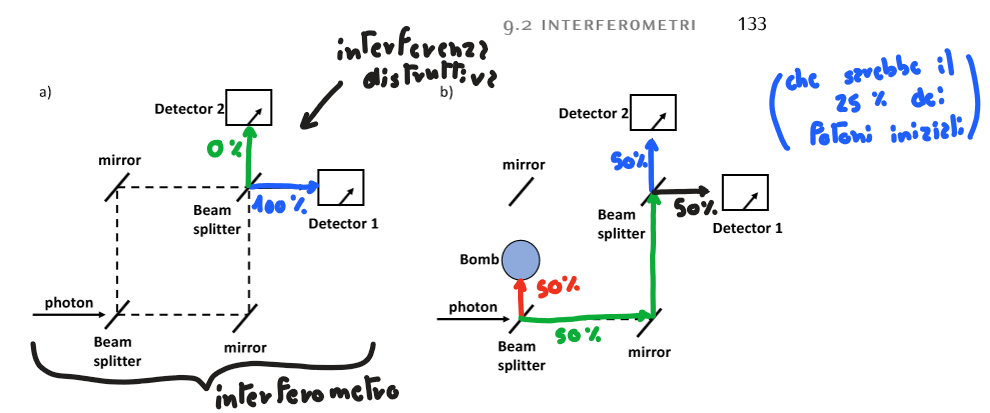
\includegraphics[width=.7\textwidth]{Immagini/interferometri.png}
\end{center}
Uno \textbf{beam splitter} è un dispositivo sulla quale un fotone avrà il 50\% di possibilità di passare in un ramo e il 50\% di passare nell'altro. Il fotone verrà poi riflesso dagli specchi e "ricombinato" dal secondo beam splitter.\\
Possiamo rappresentare i fotoni che vanno in orizzontale come $\ket{0}$ e quelli che vanno in verticale come $\ket{1}$, gli specchi come operatori $X$ e i beam splitter come porte di Hadarmard. Con queste notazioni abbiamo che la dinamica dell'interferometro in figura (a) è
\begin{equation*}
    \ket{0}\xrightarrow{H} \frac{1}{\sqrt{2}}\left(\ket{0}+\ket{1}\right)\xrightarrow{X} \frac{1}{\sqrt{2}}\left(\ket{0}+\ket{1}\right)\xrightarrow{H} \ket{0}
\end{equation*}
Adesso supponiamo che un oggetto assorbente venga posto nel ramo verticale come mostrato in figura (b). I fotoni che andranno nel ramo verticale saranno assorbiti e non arriveranno al secondo beam splitter, quindi al secondo beam splitter arriverà il 50\% dei fotoni che a sua volta dividerà. In altre parole: se un fotone (passano nel ramo inferiore) viene successivamente misurato dal detector 2, siamo sicuri che ci sia un oggetto assorbente senza che il fotone abbia interagito con esso.\\
Possiamo vedere questo fenomeno a livello più preciso introducento un terzo stato $\ket{a}$ che rappresenta il fotone assorbito.
\begin{equation*}
    \begin{split}
        \ket{0}&\xrightarrow{H}\frac{1}{\sqrt{2}}\left(\ket{0}+\ket{1}\right)\\
        &\xrightarrow{\text{assorbimento}} \frac{1}{\sqrt{2}}\left(\ket{0}+\ket{a}\right) \\
        &\xrightarrow{X}\frac{1}{\sqrt{2}}\left(\ket{1}+\ket{a}\right) \\
        &\xrightarrow{H}\frac{1}{2}\left(\ket{0}-\ket{1}\right) + \frac{1}{\sqrt{2}}\ket{a}
    \end{split}
\end{equation*}
In questo modo possiamo dire che:
\begin{itemize}
    \item Probabilità 0.25 di misurare $\ket{0}$ con il detector 1
    \item Probabilità 0.25 di misurare $\ket{1}$ con il detector 2
    \item Probabilità 0.5 di non misurare niente con i detector 
\end{itemize}
\subsection{Estensione e miglioramento}
Supponiamo di fare due modifiche all'interferometro:
\begin{enumerate}
    \item La prima è nei beam splitter che possono essere costruiti in modo tale che la maggior parte dei fotoni passi nel ramo orizzontale e soli pochi nel ramo verticale. A livello formale, questo significa che non avremo più un operatore di Hadarmard associato al beam splitter ma un generico operatore di rotazione scrivibile come \begin{equation*}
        U_{BS}(\theta) = \begin{bmatrix}
            \cos\theta & -\sin\theta \\
            \sin\theta & \cos\theta
        \end{bmatrix}
    \end{equation*} La matrice $U_{BS}(\theta)$ è una matrice di rotazione di un angolo $\theta$ nello spazio $\{\ket{0},\ket{1}\}$.
    \item La seconda modifica da apportare all'interferometro è di non misurare i fotoni dopo un passaggio ma riprendere i fotoni e farli passare attraverso $N$ beam splitter prima di misurarli. Questo equivale ad applicare l'operatore $U_{BS}(\theta)$ e quindi indurre una rotazione di un angolo $N\theta$ \begin{equation*}
        \begin{split}
            \ket{0} &\xrightarrow{U_{BS}(\theta)} \cos\theta\ket{0}+\sin\theta\ket{1} \\
            &\xrightarrow{U_{BS}(\theta)} \ldots \\
            &\xrightarrow{U_{BS}(\theta)} \cos(N\theta)\ket{0}+\sin(N\theta)\ket{1}
        \end{split}
    \end{equation*}
    A  questo punto si vede che se scegliamo $\theta = \frac{\pi}{2N}$ (quindi $\theta\ll 1$) lo stato finale sarà $\ket{1}$ e solo un detector misurerà i fotoni.
\end{enumerate}
Supponiamo adesso che la bomba sia attiva.
\begin{equation*}
    \begin{split}
        \ket{0} \xrightarrow{U_{BS}(\theta)} \cos\theta\ket{0}+\sin\theta\ket{1} &\xrightarrow{\text{assorbimento}} \cos\theta\ket{0}+\sin\theta\ket{a} \\ 
        &\xrightarrow{U_{BS}(\theta)} \cos\theta(\cos\theta\ket{0}+\sin\theta\ket{1})+\sin\theta\ket{a} \\
        &\xrightarrow{\text{assorbimento}} \cos^{2}\theta\ket{0}+(\cos\theta\sin\theta+\sin\theta)\ket{a}
    \end{split}
\end{equation*}
Estendendo questa osservazione al caso di $N$ applicazioni del beam splitter, otterremo lo stato
\begin{equation*}
    \ket{0}\xrightarrow{U_{BS}^{N}(\theta)} \cos^{N}\theta\ket{0}+(\ldots)\ket{a}
\end{equation*}
La probabilità di misurare $\ket{0}$ è:
\begin{equation*}
    P(0) = \cos^{2N}\theta = \left[\cos\left(\frac{\pi}{2N}\right)\right]^{2N} \approx \left[1-\left(\frac{\pi}{2N}\right)^{2}\right]^{2N} \approx 1-\frac{\pi^{2}}{8N} \approx 1
\end{equation*}
La probabilità di misurare $\ket{1}$ è $P(1)=\frac{\pi^{2}}{8N}\ll 1$.\\
Quindi, in presenza della bomba attiva, la probabilità di misurare $\ket{0}$ si approssima a 1 se prendiamo $\theta$ sufficientemente piccolo e $N$ (il numero di beam splitter) sufficientemente grande.\\
Riassumento: per $N$ grande, se la bomba non è attiva misureremo $\ket{1}$ (con certezza) mentre se la bomba è attiva misureremo $\ket{0}$ con una probabilità prossima a 1. Questo schema ci permette quindi di distinguere fra i due casi senza far esplodere la bomba.
\end{document}